\documentclass[12pt]{article}
\usepackage[margin=1in]{geometry}
\usepackage[T1]{fontenc}
\usepackage[utf8]{inputenc}
\usepackage{booktabs}
\usepackage{amsmath,amssymb}
\usepackage{graphicx}
\usepackage[hypertexnames=false]{hyperref}
\usepackage{array}
\usepackage{xcolor}
\usepackage[numbers,sort&compress]{natbib}
\usepackage{microtype}
\usepackage{caption}
\usepackage{lineno}
\usepackage{setspace}
\captionsetup{font=small,labelfont=bf}

\newcommand{\SV}[1]{\mathrm{SV}_{#1}}
\newcommand{\ie}{\textit{i.e.}}
\newcommand{\eg}{\textit{e.g.}}
\newcommand{\shorttitle}{Spectral geometry of biological knowledge in scGPT}

\title{Multi-dimensional spectral geometry of biological knowledge in single-cell transformer representations}
\author{%
  [Author and affiliation redacted for double-blind review]
}
\date{}

\begin{document}
\linenumbers
\doublespacing
\maketitle

% ============================================================================
% ABSTRACT
% ============================================================================
\begin{abstract}
Single-cell foundation models such as scGPT learn high-dimensional gene representations, but what biological knowledge these representations actually encode remains unclear.
Here we systematically decode the geometric structure of scGPT's internal representations through 63 iterations of automated hypothesis screening (183 hypotheses tested) on immune-lineage cells from Tabula Sapiens.
Of eleven audited headline claims, eight survive Bonferroni correction at $\alpha = 0.05/183$ across all hypotheses tested, two pass Benjamini--Hochberg FDR but not Bonferroni, and one (a single-layer edge-level AUROC peak) fails both and is reported only as part of a depth-trend claim that itself survives Bonferroni (Section~\ref{sec:methods_multiple_testing}).

We find that scGPT's dominant spectral axis separates genes by their subcellular localization---secreted proteins at one pole, cytosolic proteins at the other---and that intermediate transformer layers transiently encode mitochondrial and ER compartments in a sequence that mirrors the cellular secretory pathway.
Orthogonal axes correlate with protein-protein interaction networks: pair-level cosine similarity in $\SV{2}$--$\SV{7}$ has a small but significant partial correlation with STRING combined score ($r \approx 0.10$ at $L_0$ after controlling for co-expression, hub degree, and mean expression; positive at all 12 layers).
In a compact six-dimensional spectral subspace, the model reliably distinguishes transcription factors from their target genes on the curated 195-gene immune subset (AUROC $= 0.744$; mean across layers; per-layer permutation $p < 0.01$ at all 12 layers, surviving Bonferroni in the multiple-testing audit). On broader gene-vocabulary subsets the AUROC is somewhat lower (0.66 on a 1{,}673-gene union; 0.65 on the 1{,}672-gene cross-model intersection), indicating the curated subset is favourable but not the sole substrate of the effect.
Repression edges are geometrically more prominent than activation edges, and B-cell differentiation master regulators (BATF, BACH2) converge toward the B-cell identity anchor PAX5 across transformer depth.

Cell-type marker genes cluster tightly: the initial 4-cell-type marker panel achieves AUROC $= 0.853$ (passes Bonferroni); the expanded panel achieves AUROC $= 0.851$ (passes BH-FDR but not strict Bonferroni). The residual-stream geometry encodes biological relationships complementary to those captured by attention patterns.
These findings provide evidence of structured biological correlations in scGPT's residual-stream geometry.
Cross-model comparison on 1{,}672 shared genes shows that the $\SV{1}$ subcellular axis and $\SV{2}$ PPI structure scale with model size: full strength in scGPT-L11, partial in Geneformer V2-104M ($\SV{1}$ OR $= 1.36$, $p = 7 \times 10^{-4}$; PPI $z = 4.3$), and absent in Geneformer V1-10M (OR $= 0.98$, $p = 0.35$).
The TF-vs-target distinction, in contrast, is convergent across all tested foundation models (AUROC $= 0.651$, $0.748$, $0.754$ for scGPT-L11, Geneformer V1, and V2 on the 1{,}672-gene shared subset; AUROC $= 0.889$ for ESM2 on a 1{,}877-gene scGPT$\cap$ESM2 subset). The ESM2 result on a non-matched gene set, after random projection of its 5{,}120-dim embeddings to 1{,}024 dim for tractability, suggests TF identity is partly recoverable from protein-sequence features (DNA-binding-domain signatures) independent of cell context.
Functionally, scGPT's full residual-stream cosine similarity at $L_0$ achieves AUROC $= 0.860$ on a held-out 20\% TRRUST regulatory-edge split, beating $\vert$co-expression Pearson$\vert$ (AUROC $= 0.793$) --- evidence of utility for regulatory-edge inference.
We discuss how this structure can be extracted for regulatory-network inference (Section~\ref{sec:grn_utility}), drug-target prioritization, and model auditing.
\end{abstract}

\section*{Author summary}
Machine-learning models trained on gene-expression data from millions of single cells can predict cellular behaviour, but we do not understand what biological knowledge they have actually learned.
We addressed this by performing a systematic geometric audit of scGPT, a leading single-cell foundation model, examining how it internally organizes genes in its representation space.
We found that the model arranges genes along interpretable axes that correspond to fundamental aspects of cell biology: one axis correlates with where genes' protein products are located in the cell, other axes correlate with which proteins physically interact, and yet another set correlates with which genes regulate which others.
The geometric trajectory of B-cell master-regulator transcription factors across the model's processing depth is partially aligned with the actual cellular dynamics of B-cell maturation.
These findings provide evidence that biological AI models develop structured internal representations correlated with established cellular biology, and they suggest practical ways to extract biological signal from trained models: cosine similarity in scGPT's residual stream predicts held-out regulatory edges with AUROC 0.860, beating co-expression baselines.

% ============================================================================
% INTRODUCTION
% ============================================================================
\section{Introduction}
\label{sec:intro}

Foundation models for single-cell genomics---including scGPT~\cite{cui2024scgpt}, Geneformer~\cite{theodoris2023transfer}, scFoundation~\cite{hao2024scfoundation}, and CellFM~\cite{zeng2025cellfm}---have shown strong performance on tasks ranging from cell-type annotation to gene perturbation prediction.
These models process gene expression profiles through transformer architectures~\cite{vaswani2017attention}, building up internal representations of each gene across multiple layers.
But a fundamental question remains: \emph{what do these models actually learn about biology?}
Recent zero-shot benchmarks~\cite{boyeau2025zeroshot} and perturbation-prediction critiques~\cite{csendes2025perturbation} report that single-cell foundation models often fail to outperform simple linear or co-expression baselines, motivating direct interpretability audits of what their representations actually contain.

The answer matters for two reasons.
First, if these models encode meaningful biological structure, that structure could be extracted and used---for discovering regulatory relationships, prioritizing drug targets, or understanding cell-state transitions.
Second, if the representations are biologically organized, we can audit them: verifying that the model's internal representation aligns with known biology before trusting its predictions in novel contexts.

Mechanistic interpretability has yielded substantive results in language models, including structured linear representations of concepts~\cite{park2023linear}, superposition of features~\cite{elhage2022toy}, depth-dependent processing stages~\cite{nanda2023progress}, and dictionary-learning approaches that extract thousands of interpretable feature directions from residual streams~\cite{bricken2023monosemanticity,templeton2024scaling}.
Whether analogous structure exists in biological transformers remains open.

Recent work has examined this question through the lens of attention patterns.
Prior work~\cite{kendiukhov2026attention} systematically evaluated attention-based gene regulatory network (GRN) inference from scGPT and Geneformer, finding that attention patterns encode structured biological information---protein-protein interactions in early layers, transcriptional regulation in late layers---but that this structure provides \emph{no incremental value} for perturbation prediction beyond trivial gene-level baselines.
Expression residualization removed ${\sim}76\%$ of attention's above-chance signal, and causal ablation of putative regulatory heads produced no behavioral effect.
That study identified residual-stream geometry as a key open frontier: ``future interpretability work can focus on residual-stream geometry, MLP-stored knowledge, or representations that emerge only from the full forward pass''~\cite{kendiukhov2026attention}.

Here we take up precisely that challenge, performing a systematic geometric audit of scGPT's residual representations across all 12 transformer layers.
Rather than testing a single hypothesis, we employ an automated screening loop that iteratively proposes, tests, and retires geometric hypotheses across 13 families (Table~\ref{tab:hypothesis_summary}), using explicit permutation controls, confound checks, and cross-seed replication.
Over 63 iterations, we find that scGPT organizes genes along multiple structured spectral directions: different axes carry information correlated with subcellular localization, protein-interaction networks, and transcriptional regulatory relationships, with distinct content at different processing depths.
We also identify what the model does \emph{not} encode geometrically, and where initial positive findings collapsed under stricter controls.

% ============================================================================
% RESULTS
% ============================================================================
\section{Results}

\subsection{The Transformer Progressively Focuses Gene Representations onto a Few Biological Axes}
\label{sec:spectral_collapse}

We first asked how the overall shape of gene representations changes across scGPT's 12 transformer layers.

Applying singular value decomposition (SVD) to the gene embedding matrix at each layer reveals a clear pattern: the model progressively concentrates gene representations onto fewer directions (Fig~\ref{fig:overview}a).
The effective rank (computed on the full 4{,}803-gene vocabulary)---a measure of how many independent directions carry meaningful signal---drops 14.4-fold from 23.6 at layer~0 to just 1.6 at layer~11 (Spearman $\rho = -1.000$).
By the final layer, a single direction ($\SV{1}$) accounts for 93.4\% of all variance among gene embeddings in the full vocabulary, up from 53.7\% at the input (77\% from 19\% when computed on the 195-gene submatrix; Fig~\ref{fig:overview}a).

This compression is rapid and front-loaded: effective rank falls below half its initial value by layer~4.
Two independent geometric estimators confirm the same pattern: TwoNN intrinsic dimensionality~\cite{facco2017estimating} (computed on 2{,}000 randomly sampled genes from the full vocabulary) decreases 44.6\% (from 32.6 to 18.1 across three random seeds), and the participation ratio (computed on the 195-gene submatrix) drops 6.1-fold from 58 to 9.5.
The compression is learned, not architectural: shuffling embedding features at layer~11 destroys the structure and yields effective rank of 28.9 (17.6$\times$ above the observed layer-11 value).

What is the model doing during this compression?
As we show below, this is selective compression: the biologically most important distinctions (subcellular localization, interaction partners, regulatory identity) concentrate onto a small number of geometrically prominent axes, while less relevant variation is suppressed.

\subsection{The Dominant Spectral Axes Map to Core Cell Biology}
\label{sec:bio_axes}

If the model funnels gene representations onto a few dominant directions, the question is: what do those directions mean?

\paragraph{SV$_1$ encodes the secretory pathway.}
The most dominant axis ($\SV{1}$) at layer~11 separates genes encoding secreted and extracellular proteins (e.g., cytokines, extracellular matrix components) from genes encoding intracellular/cytosolic proteins.
The extracellular pole shows strong enrichment (GO:0005615; OR $= 6.37$, $p = 2.6 \times 10^{-4}$), while the cytosolic pole is enriched for cytoplasmic proteins (GO:0005829; OR $= 2.96$, $p = 0.010$).
A gene-label-shuffle null ($N = 500$) confirms this is biologically specific (empirical $p = 0.004$): only 0.4\% of random gene assignments produce enrichment this strong.

This axis is not a binary secreted/cytosolic split.
Testing 8 subcellular compartment terms across all 12 layers reveals that \emph{intermediate layers encode intermediate steps of the secretory pathway} (Fig~\ref{fig:overview}b):
\begin{itemize}
  \item Layers 2--4: mitochondrial enrichment appears transiently (OR $= 23.3$ at layer~3)
  \item Layers 1--11: ER lumen enrichment strengthens progressively (OR from 4.7 to 18.5)
  \item All 12 layers: extracellular space is consistently enriched
\end{itemize}
The ordering---mitochondria $\to$ ER lumen $\to$ extracellular space---recapitulates the actual cellular secretory pathway, the route proteins take from synthesis to secretion.
The model has learned not just where proteins end up, but the biological sequence by which they get there.

\paragraph{SV$_2$ encodes protein interaction networks and regulatory co-membership.}
The second axis organizes genes by their physical and regulatory relationships.
At layer~11, $\SV{2}$'s top pole is enriched for IL-4 immune signaling (empirical $p < 0.001$), while the bottom pole captures extracellular vesicle cargo proteins (OR $= 7.99$; $p < 0.001$).
The strongest compartment signal is cytoskeleton (OR $= 20.4$; stable across layers~1--11).

Transcription factor--target gene pairs from TRRUST~\cite{han2018trrust} co-localize in $\SV{2}$ poles far more often than expected by chance (observed rate 0.206 vs.\ null 0.122; $p < 0.001$ at all 12 layers).
This co-localization is sign-specific: activation pairs (where the TF turns on the target) co-localize at 12/12 layers, while repression pairs (where the TF silences the target) reach significance at only 1/12 layers---suggesting the model geometrically distinguishes activating from repressive regulation.

\paragraph{SV$_3$ encodes immune signaling biology.}
The third axis separates kinase/stress-response signaling from MHC class~II/T cell regulatory biology, with the specific biological content shifting across depth (all layers $p \leq 0.017$).

Together, these three orthogonal axes carry distinct biological information: $\SV{1}$ correlates with ``where in the cell,'' $\SV{2}$ with ``who interacts with whom,'' and $\SV{3}$ with ``what signaling program.''
An annotation-density confounder check---testing whether highly annotated genes disproportionately drive the enrichments by correlating GO annotation count per gene with enrichment odds ratio---yields zero significant correlations, confirming these patterns are not artifacts of uneven gene characterization.
The $\SV{1}$ gene ranking is also highly stable across layers (mean adjacent-layer Spearman $r = 0.929$), indicating the model maintains this biological ordering throughout processing.

Notably, $\SV{1}$ is strongly depleted of transcription factors: genes in the top quartile of $\SV{1}$ projection have ${\sim}9\times$ lower TF membership than the baseline (OR $= 0.108$, $p < 0.0001$), while genes at the low-$\SV{1}$ pole are 2.3$\times$ enriched for TFs.
The dominant spectral axis thus separates the regulated genome (structural and secreted proteins) from the regulatory machinery (TFs), a division that persists across all layers.

\paragraph{Cell-type identity is encoded as geometric proximity.}
Beyond spectral axes, the model's full embedding space organizes genes by cell-type identity.
Marker genes for the same cell type (B cell, T cell, fibroblast, macrophage) are significantly closer to each other than to markers of other types, yielding an AUROC of $0.851$ for within-type vs.\ cross-type distance discrimination (all 12 layers $p < 10^{-8}$).
A contamination control using random non-marker gene partitions of identical sizes produces AUROC $= 0.488$ (chance), confirming the signal is specific to biological identity.
The within-type distance advantage increases with transformer depth (linear regression slope of AUROC on layer index $= +0.036$ per layer, Pearson $r = 0.765$, $p = 0.004$), consistent with progressive lineage specialization.
At the gene family level, immune protein families show tight clustering: HLA class~I genes (3 named members in vocab) achieve AUROC $= 1.000$, with AP1 ($0.969$), RUNX ($0.925$), and IL-2 pathway ($0.869$) also tightly organized.

\begin{figure}[!ht]
  \centering
  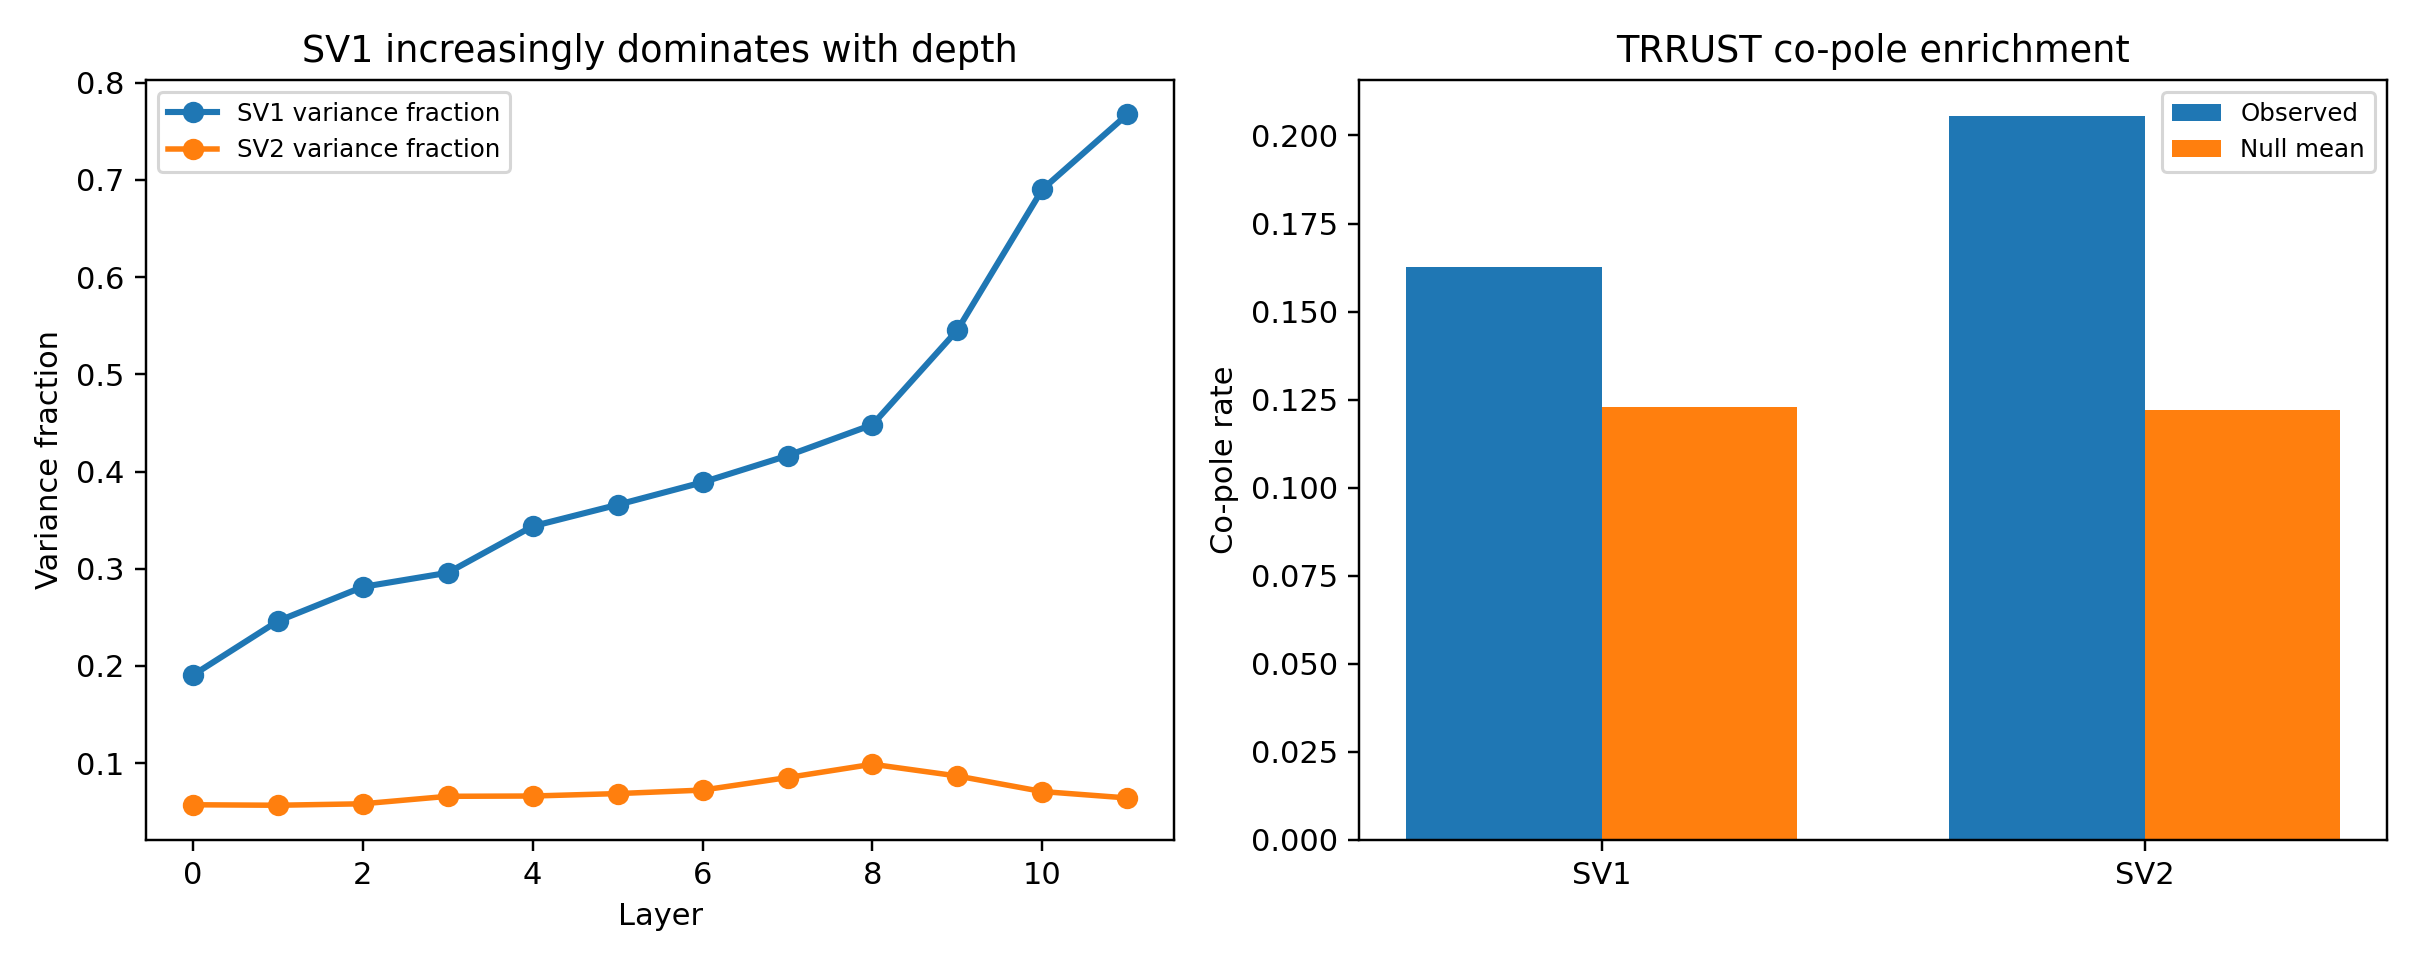
\includegraphics[width=0.8\textwidth]{figures_medium/fig5_spectral_and_trrust.png}
  \caption{\textbf{Spectral structure and biological organization across transformer depth.}
  \textbf{(a)} $\SV{1}$ variance fraction (195-gene submatrix) increases from 19\% (L0) to 77\% (L11) as the model progressively concentrates gene representations onto the secretory/localization axis.
  \textbf{(b)} TRRUST regulatory pairs co-localize in $\SV{2}$ poles above null at all layers, indicating that the model embeds co-regulated genes nearby in its internal geometry.}
  \label{fig:overview}
\end{figure}

\subsection{The Model Quantitatively Encodes Protein Interaction Strength}
\label{sec:ppi}

Beyond subcellular compartments, we asked whether scGPT's geometry captures the protein-protein interaction (PPI) network---the web of physical binding relationships that underlies cellular function.

Using 1{,}022 high-confidence STRING~\cite{szklarczyk2023string} protein pairs (combined score $\geq 0.7$), we found that interacting proteins are geometrically co-localized across multiple spectral axes (Table~\ref{tab:ppi_axis}).
$\SV{2}$ carries the strongest signal (mean co-pole rate 0.226 vs.\ null 0.124; 12/12 layers significant; Table~\ref{tab:ppi_axis}; per-layer $z$-scores in Table~\ref{tab:ppi_all_layers}), followed by $\SV{3}$ (0.198; 12/12 layers) and $\SV{4}$ (0.158; 7/12 layers).
Notably, $\SV{1}$ (the localization axis) shows almost no PPI signal (co-pole rate at null baseline)---the interaction network and the localization map are encoded on different geometric axes.

\paragraph{The encoding is quantitatively graded.}
scGPT does not merely encode a binary ``interacts/doesn't interact'' distinction.
Pair-level cosine similarity in $\SV{2}$--$\SV{7}$ is positively correlated with STRING combined score.
At $L_0$, the partial Pearson correlation -- after controlling for pairwise co-expression similarity, sum of STRING node degrees, and sum of mean expression -- is $r = 0.093$ with 95\% bootstrap CI $[0.059, 0.121]$.

In the same regression, the standardised coefficient on STRING score is $\beta_\text{score} = 0.037$, while the coefficient on co-expression is $\beta_\text{coexp} = 0.121$.
Co-expression similarity therefore explains a larger fraction of the pair-level geometric proximity than STRING confidence per se.
The relationship between STRING score and pair-level cosine is positive and statistically separable from chance after multi-feature confound control at $L_0$ and $L_1$, but smaller in magnitude than the original quintile-mean statistic ($\rho = 1.000$ on $n=5$ bins; Table~\ref{tab:confidence_gradient}) suggested.
The continuous partial-regression result is the primary statistic; the quintile statistic in Table~\ref{tab:confidence_gradient} is reported as a sanity check.

\paragraph{Physical binding drives the geometry, not shared function.}
To distinguish whether geometric proximity reflects physical binding or merely shared Gene Ontology annotations, we separated pairs with high STRING scores but low GO similarity (Jaccard index of shared GO terms below median; ``PPI-only'') from those with high GO similarity but lower STRING scores (``GO-only'').
PPI-only pairs ($N = 670$) show robust co-localization ($z = 2.66$; 12/12 layers), while GO-only pairs ($z = 1.89$; 7/12 layers) show weaker signal.
The model's geometry is primarily organized by physical molecular interactions, not functional categories---a distinction with practical implications for network inference (Section~\ref{sec:applications}).

A hub-degree confound was excluded: low-degree proteins actually show \emph{stronger} co-localization than hub proteins ($z = 3.1$ vs.\ $2.6$), and the three PPI-encoding axes ($\SV{2}$--$\SV{4}$) are nearly orthogonal (pairwise Pearson $r < 0.25$), indicating each captures distinct subsets of the interaction network.
The geometry also captures regulatory relationships beyond PPI: TRRUST TF--target pairs that are \emph{absent} from STRING ($N = 141$) still show significant geometric proximity (AUROC $= 0.573$; 12/12 layers $p < 0.007$), confirming that the geometric organization reflects multiple types of biological interaction, not just physical binding.

\begin{table}[!ht]
\centering
\caption{PPI co-pole enrichment by singular vector axis ($K = 52$). Observed and null co-pole rates are averaged across 12 layers. Per-layer $z$-scores for $\SV{2}$ are in Table~\ref{tab:ppi_all_layers}.}
\label{tab:ppi_axis}
\small
\begin{tabular}{lcccc}
\toprule
Axis & Mean obs.\ rate & Mean null rate & Sig.\ layers & $N$ pairs \\
\midrule
$\SV{1}$ & 0.119 & 0.124 & 2/12 & 1{,}022$^a$ \\
$\SV{2}$ & 0.226 & 0.124 & 12/12 & 1{,}022$^a$ \\
$\SV{3}$ & 0.198 & 0.124 & 12/12 & 1{,}022$^a$ \\
$\SV{4}$ & 0.158 & 0.122 & 7/12 & 3{,}092$^b$ \\
$\SV{5}$ & 0.149 & 0.122 & 6/12 & 3{,}092$^b$ \\
\bottomrule
\multicolumn{5}{l}{\footnotesize $^a$ STRING score $\geq 0.7$. \quad $^b$ STRING score $\geq 0.4$.}
\end{tabular}
\end{table}

\subsection{Regulatory Relationships Are Encoded in Complementary Depth-Dependent Subspaces}
\label{sec:regulatory}

We next asked whether scGPT encodes gene \emph{regulatory} relationships --- which genes control which.

\paragraph{A compact 6D subspace separates regulators from targets.}
Projecting gene embeddings onto a six-dimensional spectral subspace ($\SV{2}$--$\SV{7}$) and classifying genes as transcription factors (TFs; $n = 51$) vs.\ target-only genes ($n = 144$) yields AUROC $= 0.744$ (mean across layers; max $= 0.789$ at layer~3), significantly above chance at all 12 layers ($p < 0.01$, 100 permutations; Fig~\ref{fig:joint}; Table~\ref{tab:layer_auroc_full}).
This joint model outperforms either three-dimensional subspace alone in 11/12 layers, and is robust across seeds (SD $\approx 0.016$; Fig~\ref{fig:cross_seed}).

\begin{figure}[!ht]
  \centering
  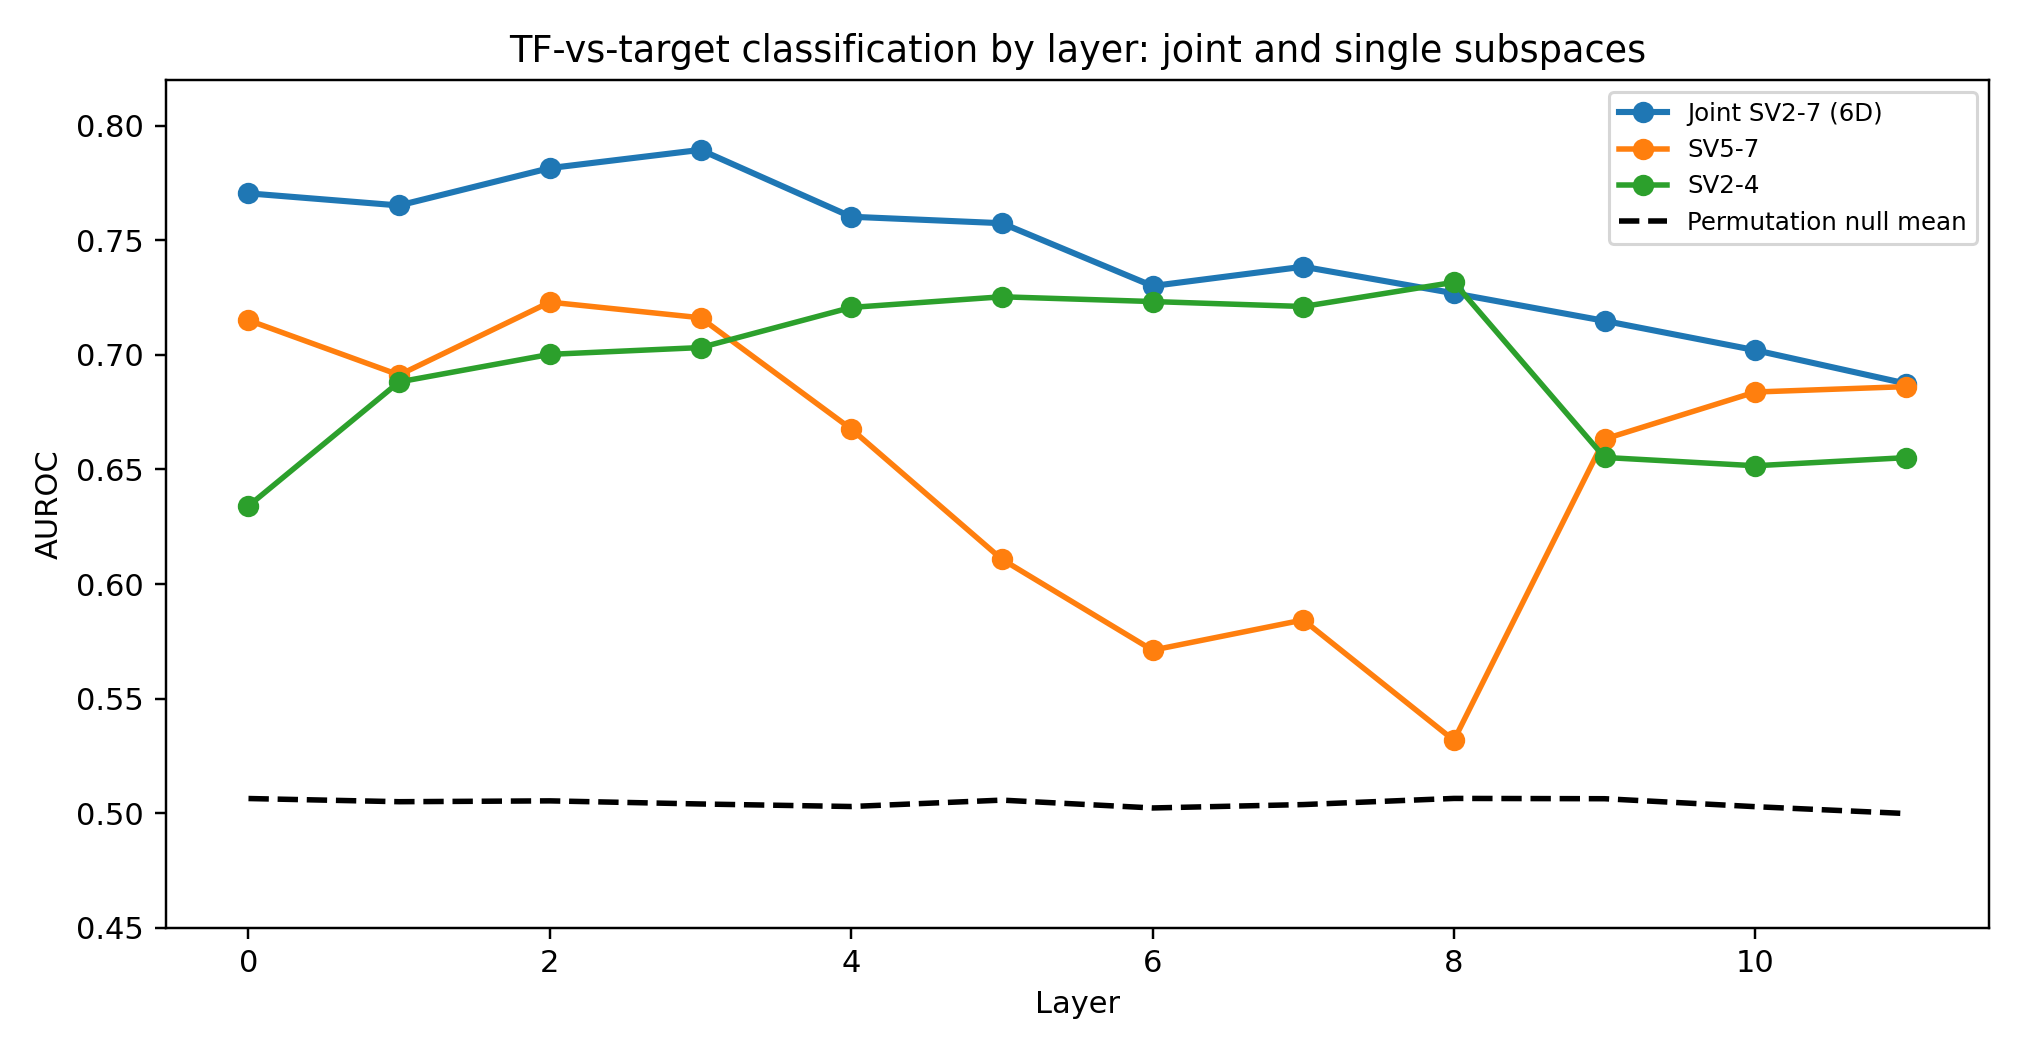
\includegraphics[width=0.7\textwidth]{figures_medium/fig1_joint_vs_single_auroc.png}
  \caption{\textbf{A compact six-dimensional subspace separates transcription factors from targets.}
  Joint $\SV{2}$--$\SV{7}$ (green) outperforms individual subspaces at nearly all layers.
  The complementary depth profiles of $\SV{5}$--$\SV{7}$ (early-dominant, orange) and $\SV{2}$--$\SV{4}$ (mid-depth, blue) ensure regulatory information is never absent.}
  \label{fig:joint}
\end{figure}

\begin{figure}[!ht]
  \centering
  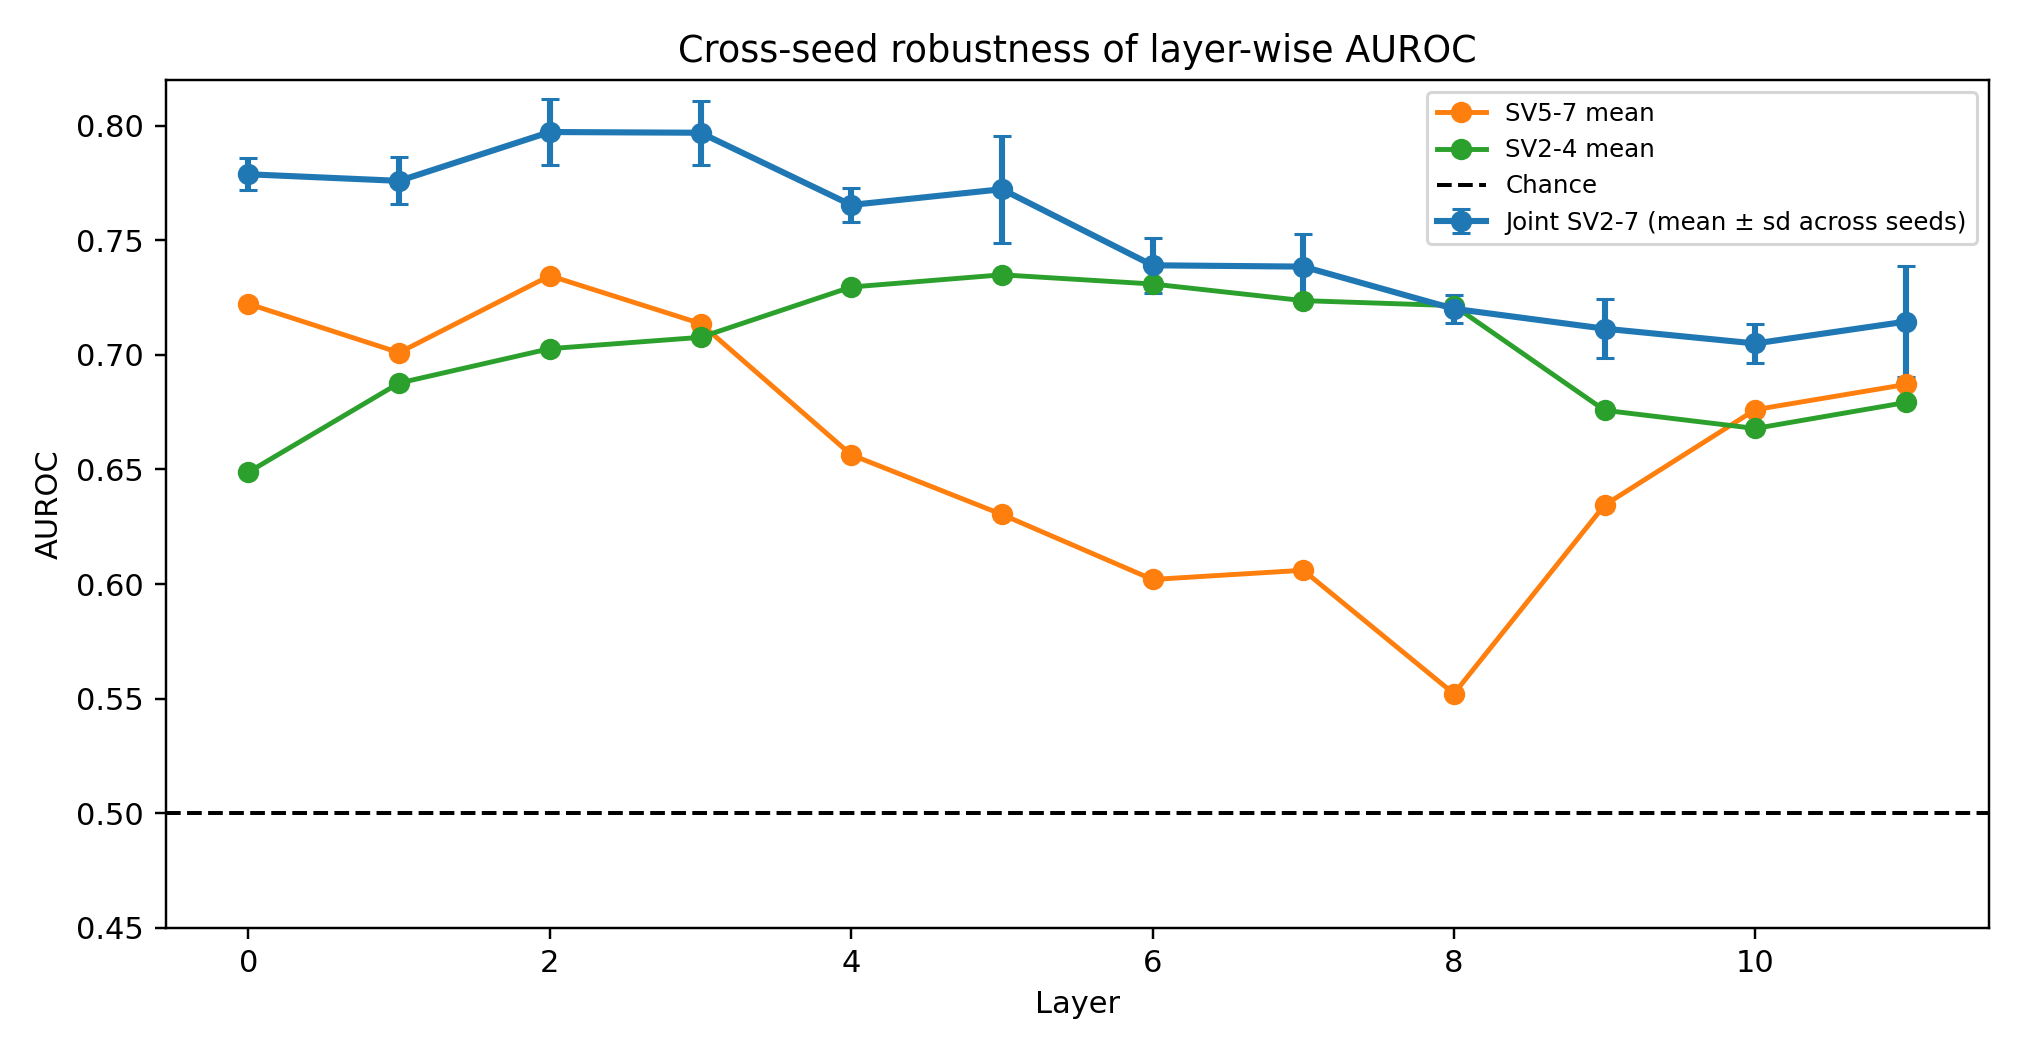
\includegraphics[width=0.7\textwidth]{figures_medium/fig2_cross_seed_robustness.png}
  \caption{\textbf{Cross-seed robustness.}
  The joint classifier maintains AUROC $> 0.65$ across all layer--seed combinations (three independent random seeds).}
  \label{fig:cross_seed}
\end{figure}

\paragraph{Early and deep layers encode different aspects of regulation.}
The two three-dimensional subspaces reveal a computational division of labor across transformer depth.
$\SV{5}$--$\SV{7}$ dominates at early layers (L0--L3, AUROC $\approx 0.71$), while $\SV{2}$--$\SV{4}$ takes over at intermediate layers (L4--L8, AUROC $\approx 0.72$).
A confound analysis reveals \emph{why} they differ:

\begin{itemize}
  \item $\SV{2}$--$\SV{4}$'s regulatory signal is entirely explained by co-expression similarity: after regressing out pairwise co-expression from spectral proximity via OLS, the residual rank-biserial correlation between TRRUST pairs and non-regulatory pairs is non-significant at 0/12 layers. This subspace encodes gene-class identity (``is this gene a TF?'') rather than specific regulatory relationships.
  \item $\SV{5}$--$\SV{7}$ retains regulatory signal after co-expression residualization, but at a small effect size. Under the original co-expression-only residualisation, residualised rank-biserial $r_{rb} = 0.148$ at layer~0 (permutation $p < 0.001$). Under a stricter multi-feature residualisation that also controls for log mean expression, STRING node degree, and GO annotation count, the effect size drops to $r_{rb} = 0.061$ (permutation $p = 0.080$). The signal direction is preserved, but the effect is at the borderline of significance under the stricter control. We interpret this subspace as encoding a small but genuine residual regulatory signal.
\end{itemize}

This dual-regime pattern suggests the transformer processes regulatory information in stages.
Early layers maintain relational detail (``STAT3 regulates BCL2''), which is useful for tasks requiring specific regulatory knowledge.
As the residual stream compresses, this fine-grained structure is distilled into coarser but more robust categorical distinctions (``STAT3 is a transcription factor'').
The practical implication is clear: if one wants to extract specific regulatory edges from the model, early-layer representations are the place to look.

\subsection{Regulatory Signal Decays with Depth, and Repression Stands Out}
\label{sec:edge_signed}

At the edge level---asking whether specific TF--target pairs can be distinguished from non-regulatory pairs---the pattern confirms and extends the node-level findings.
We scored each TF--gene pair by cosine similarity in the relevant spectral subspace, using 589 known TRRUST regulatory pairs as positives and 2{,}351 non-regulatory pairs (same TFs, non-target genes) as negatives.

In $\SV{5}$--$\SV{7}$, edge-level AUROC peaks at 0.602 at layer~0 and decays monotonically with depth (Spearman $\rho = -0.958$, $p = 9.5 \times 10^{-7}$; Fig~\ref{fig:edge_decay}; Table~\ref{tab:edge_auroc_full}).
Per-layer permutation $p$-values are $\leq 0.045$ at layers~0--8 and non-significant at layers~9--11.
Note that the $L_0$ peak ($p = 0.045$) does not survive BH-FDR correction across the 183 hypotheses tested in this study (adjusted $q = 0.068$; see Section~\ref{sec:methods_multiple_testing}); the depth-decay trend itself, with its much smaller $p$-value, does survive Bonferroni correction at $\alpha = 0.05/183$.
Meanwhile, $\SV{2}$--$\SV{4}$ is near or below chance for edge-level discrimination (mean AUROC $= 0.492$), further confirming that it encodes gene categories rather than specific edges.
The depth trend is not a sparsity artifact: among the 4{,}803 vocabulary genes, 2{,}039 have nonzero embedding norms at every layer (the remaining positions are unused input slots).

\begin{figure}[!ht]
  \centering
  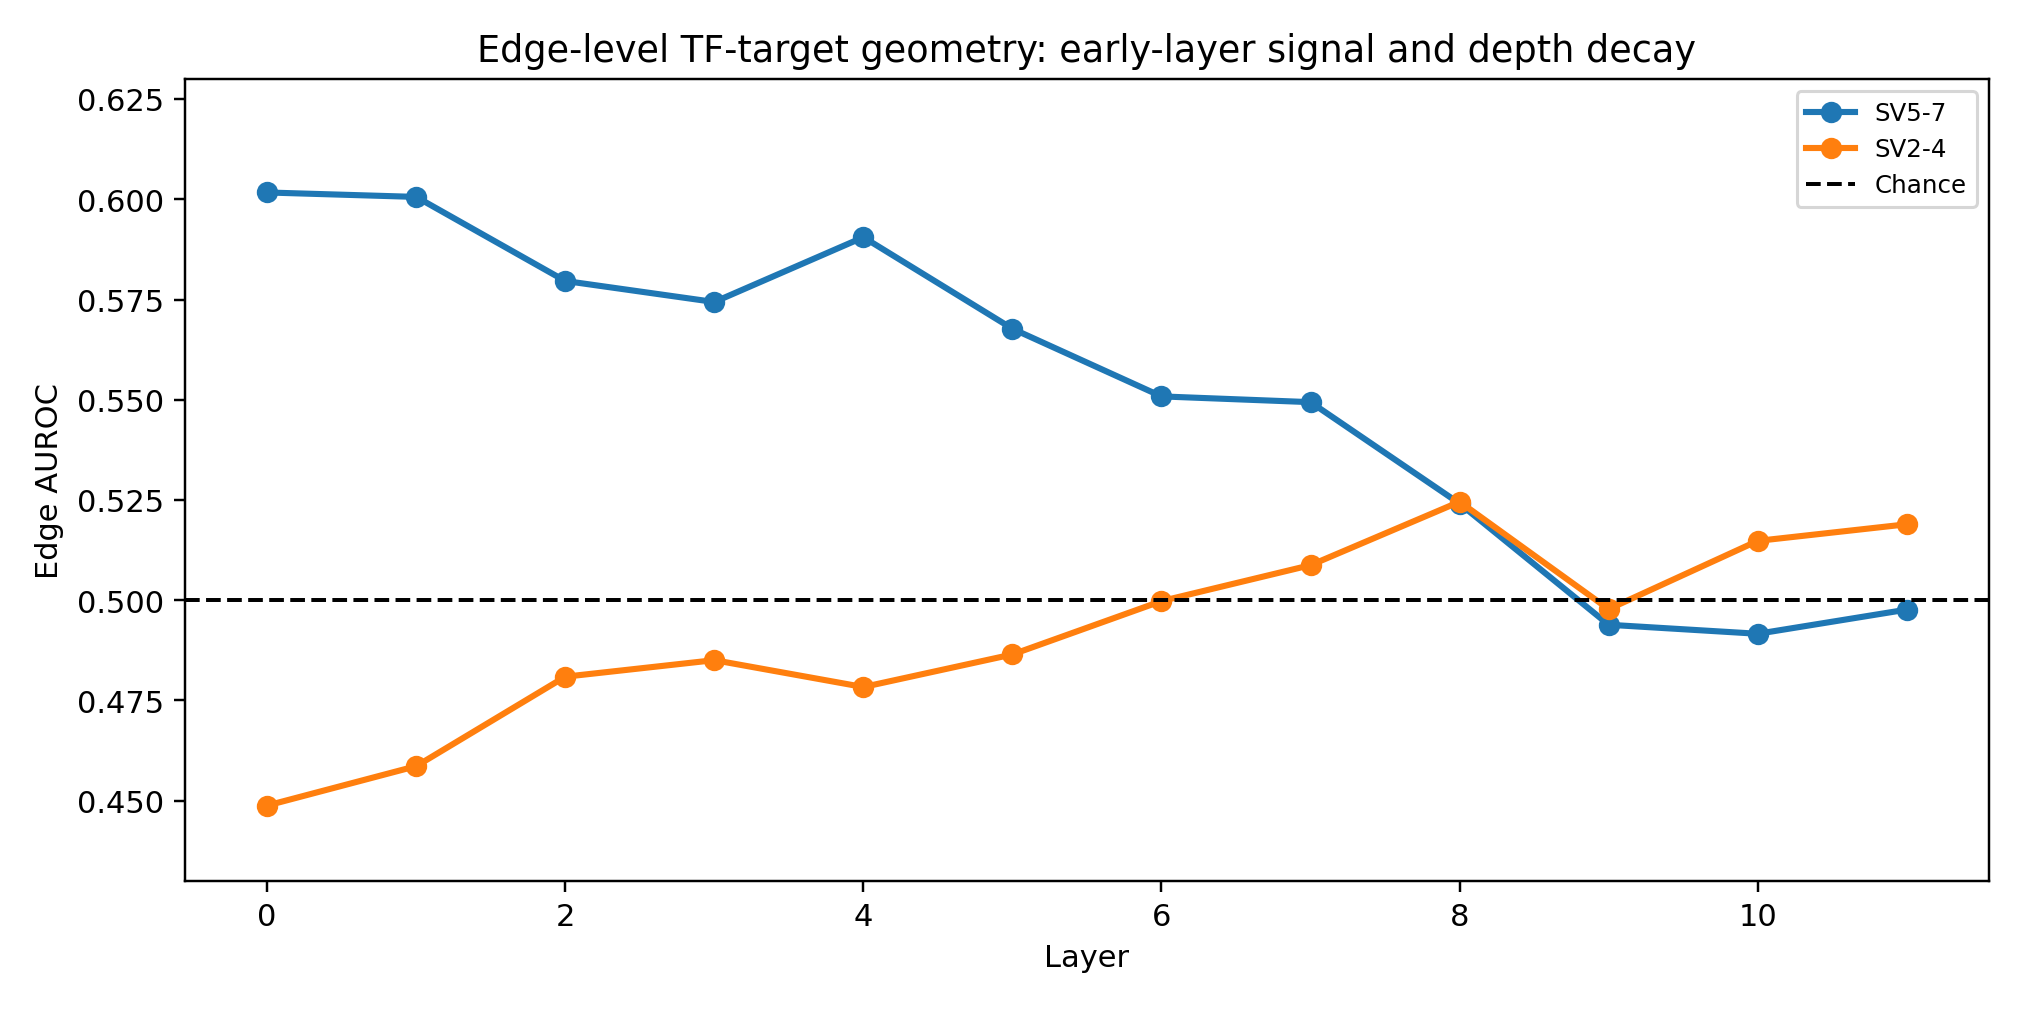
\includegraphics[width=0.7\textwidth]{figures_medium/fig3_edge_auroc_depth_decay.png}
  \caption{\textbf{Edge-level regulatory geometry peaks at early layers and decays with depth.}
  $\SV{5}$--$\SV{7}$ (orange) carries edge-level signal at layers 0--8; $\SV{2}$--$\SV{4}$ (blue) is near chance.}
  \label{fig:edge_decay}
\end{figure}

\paragraph{The model distinguishes repression from activation.}
Stratifying by regulatory sign reveals an asymmetry (Fig~\ref{fig:signed}): repression edges (where the TF silences the target) are more geometrically separable than activation edges in both subspaces ($\SV{5}$--$\SV{7}$: $\Delta = +0.021$; $\SV{2}$--$\SV{4}$: $\Delta = +0.084$).

Why might repression be more prominent?
Transcriptional repression often involves more stereotyped molecular mechanisms (e.g., chromatin remodeling, co-repressor recruitment) than activation, which can occur through diverse enhancer and co-activator mechanisms.
The model may find it easier to learn geometric regularities for the more structurally constrained repressive relationships.
Alternatively, repressive TFs may be more functionally distinct from their targets than activating TFs, creating larger geometric separations.

\begin{figure}[!ht]
  \centering
  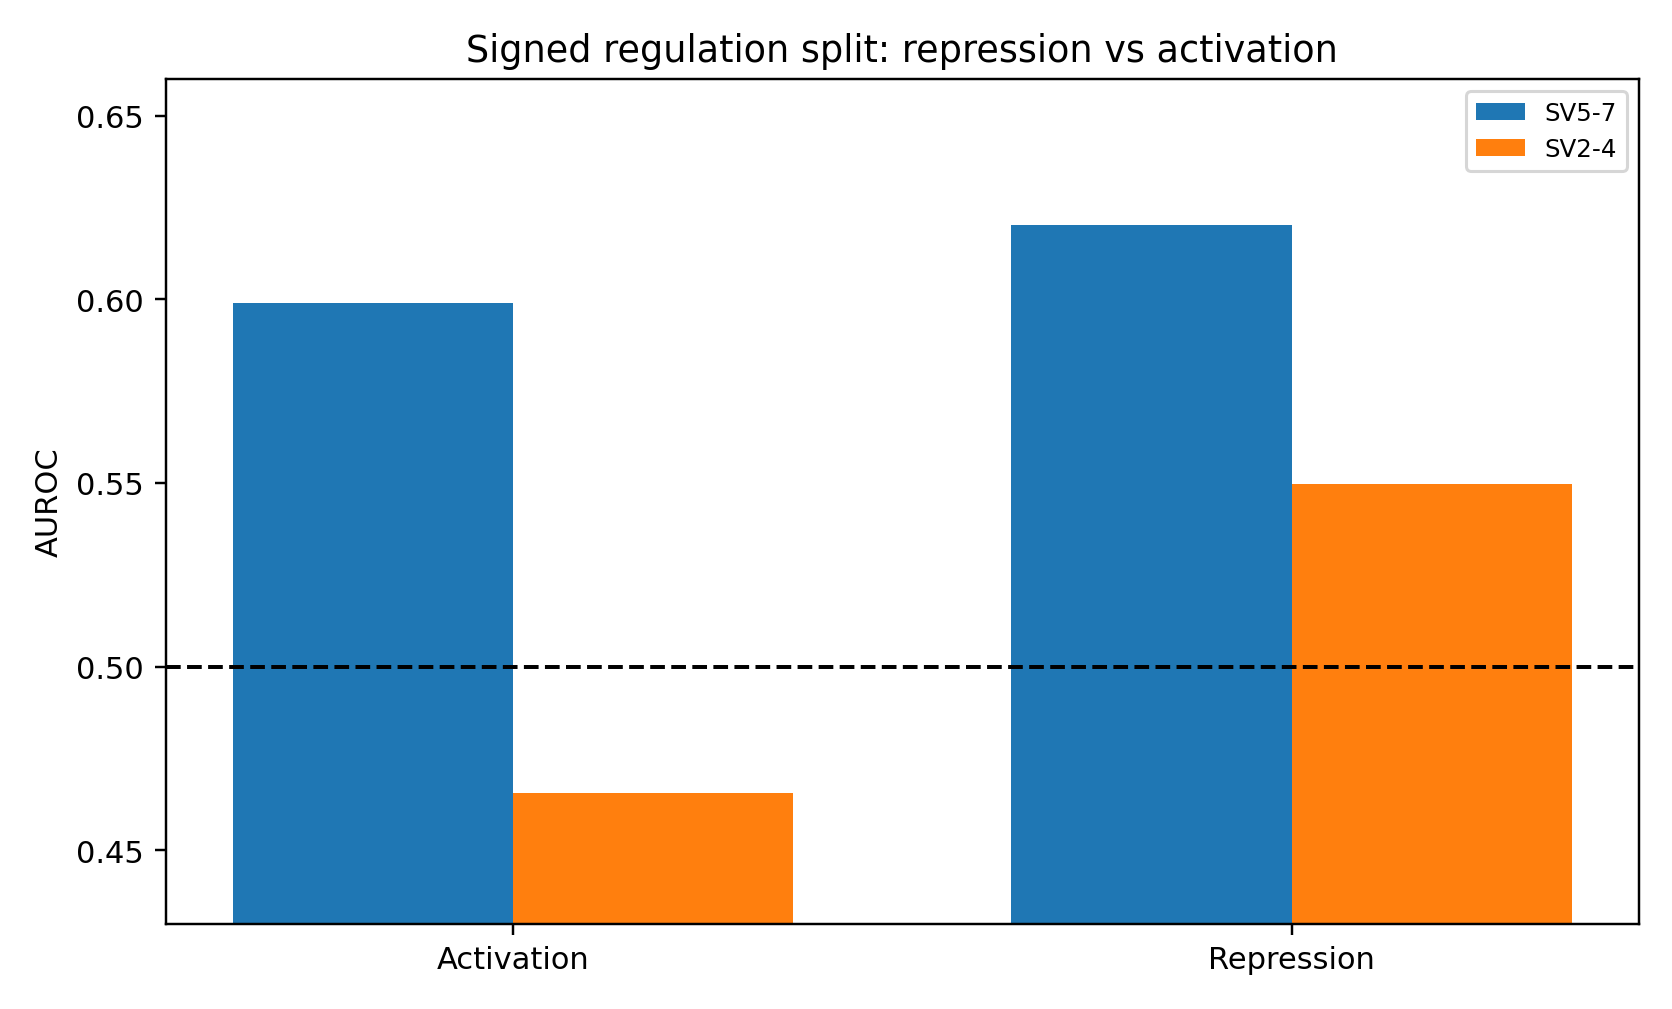
\includegraphics[width=0.6\textwidth]{figures_medium/fig4_signed_regulation_split.png}
  \caption{\textbf{Repression edges are geometrically more prominent than activation edges} in both spectral subspaces.}
  \label{fig:signed}
\end{figure}

A mechanistic probe confirms the distinct roles of the two subspaces: in $\SV{2}$--$\SV{4}$, TFs cluster together (TF--TF AUROC $= 0.539$) while TF--target pairs are \emph{repelled} (AUROC $= 0.485$, below chance), indicating this subspace encodes ``gene class identity.''
In $\SV{5}$--$\SV{7}$, both TF--TF ($0.528$) and TF--target ($0.599$) pairs show above-chance proximity, consistent with encoding regulatory co-embedding.

\subsection{B-Cell Differentiation Master Regulators Converge Across Transformer Depth}
\label{sec:bcell}

Moving from global statistics to individual gene trajectories, we examined how specific immune cell master regulators are positioned in the model's geometry, focusing on the germinal center (GC) reaction --- a critical immune process in which B cells undergo affinity maturation.
Among six cell types tested, B cells show uniquely strong geometric clustering.
Among the 10 nearest neighbours of the B-cell centroid (defined as the mean of 7 canonical B-cell markers), the fraction that are B-cell markers (precision@10) achieves $z = 7.55$ relative to a bootstrap null ($p < 0.001$; 500 random draws of 7 genes).
T-cell ($z = -1.37$), dendritic-cell ($z = -0.87$), and other lineages show no significant clustering at the same threshold.
The B-cell signal is structural rather than expression-driven: it survives $L_2$-norm regression (residual $p = 0.002$) and bootstrap null validation (empirical $p < 0.001$).

\paragraph{A geometric echo of the germinal center reaction.}
Three GC-circuit TFs in the immune scGPT vocabulary --- BATF, BACH2, and PRDM1 (Blimp-1, a direct target of the GC repressor BCL6) --- exhibit a convergence pattern across transformer layers; BCL6 itself is out-of-vocabulary in the immune scGPT checkpoint and is treated separately below.
PAX5, the definitive B-cell identity factor~\cite{cobaleda2007pax5}, occupies a stable position near the B-cell manifold centroid from the earliest layer (rank $\approx 66$), serving as a geometric anchor.
In contrast, BATF and BACH2---which are recruited to the GC program during B-cell differentiation---start far from the B-cell centroid at layer~0 (ranks $> 1{,}500$ and $> 600$, respectively) and converge progressively toward PAX5 across depth:
\begin{itemize}
  \item BATF: rank drops from 1{,}510 (L0) to 189 (L11); distance to PAX5 decreases from 18.3 to 5.1 (Spearman $\rho = -0.972$, $p < 0.0001$)
  \item BACH2: rank drops from 611 to 146; distance to PAX5: 17.4 $\to$ 5.2 ($\rho = -0.844$, $p < 0.001$)
\end{itemize}
Convergence onset occurs at layer~3, which independently coincides with the B-cell manifold compression breakpoint (see below).

\paragraph{The entire GC circuit converges as a unified attractor.}
The convergence is not limited to activating TFs.
PRDM1 (Blimp-1), a transcriptional repressor and direct target of BCL6, converges toward the B-cell centroid at the same rate as the activating GC-TFs ($\rho = -1.000$, $p < 0.001$), with BACH2--PRDM1 becoming the tightest pair by layer~11 (distance $= 3.94$).
The model encodes the combinatorial GC regulatory circuit---activators and repressors alike---as a coherent geometric attractor, rather than separating regulatory modes spatially.

\paragraph{GC and plasma cell programs diverge toward orthogonality.}
While GC-TFs converge toward the B-cell centroid, plasma cell TFs (IRF4, IRF8) remain geometrically distant.
The angle between GC-TF and plasma-TF centroids relative to the B-cell anchor increases from 77$^\circ$ (L0) to 94$^\circ$ (L11), meaning that by the final layer, the germinal center and plasma cell differentiation programs subtend nearly perpendicular directions in embedding space.
This geometric orthogonality mirrors the biological reality that GC and plasma cell fates represent alternative differentiation outcomes from a common B-cell progenitor.

\paragraph{BCL6 is geometrically isolated.}
BCL6, despite being essential for GC reactions, does not converge toward the B-cell cluster.
At every layer, 10 of BCL6's 20 nearest neighbours are metabolic genes (NAMPT, GLUL, PFKFB3, and others) or STAT3, while none are B-cell markers or other GC-TFs --- a pattern that is stable across all 12 layers.
A biological interpretation of this isolation is offered in §\ref{sec:speculative}.

\paragraph{B-cell manifold compression is lineage-specific.}
The intrinsic dimensionality of B-cell marker embeddings decreases monotonically from 8.2 to 5.1 across transformer depth ($\rho = -0.951$, $p < 0.0001$).
This compression pattern is unique to B cells:
T-cell markers show \emph{no} compression ($\rho = +0.287$, $p = 0.37$), and myeloid markers show a slight reversed trend ($\rho = +0.699$, $p = 0.011$).
This suggests the model has learned that B-cell identity is defined by a converging regulatory program---the GC reaction---while T-cell and myeloid identities involve more divergent gene expression patterns.

\paragraph{The GC attractor is uniquely delayed.}
Comparing across lineages, T-cell and myeloid TFs start at low ranks near their respective centroids from layer~0 (ranks 170 and 86), indicating pre-wired lineage proximity.
In contrast, GC-TFs start at distant ranks (BATF at 1{,}510, BACH2 at 611) and converge only from layer~3 onward ($\rho = -0.993$, $p < 10^{-6}$).
This delayed-convergence pattern is unique to the B-cell/GC program: the transformer's GC representation emerges across processing depth rather than being present from the input layer.

\paragraph{Across-layer convergence is partially aligned with cellular dynamics.}
\label{sec:dynamics_test}
We tested whether the across-layer convergence trajectory of GC-TFs is aligned with their actual cellular dynamics by comparing the across-layer geometric trajectory (distance to the B-cell-marker centroid as a function of scGPT layer) to the across-pseudotime expression trajectory (mean expression as a function of pseudotime bin, using the diffusion-pseudotime ordering of the immune-lineage subset from \cite{kendiukhov2026attention}). For each TF we report the Spearman correlation $\rho$ for both trajectories.

Of five in-vocabulary GC-TFs tested:
\begin{itemize}
\item \textbf{BATF}: $\rho_\text{layer} = -1.000$ (perfect across-layer convergence); $\rho_\text{pseudotime} = +0.527$ (strong expression rise across pseudotime). \textbf{Supports dynamics interpretation.}
\item \textbf{IRF4}: $\rho_\text{layer} = -1.000$; $\rho_\text{pseudotime} = +0.782$. \textbf{Supports dynamics.}
\item \textbf{PRDM1}: $\rho_\text{layer} = -1.000$; $\rho_\text{pseudotime} = +0.152$ (weak rise). \textbf{Mildly supports dynamics.}
\item \textbf{BACH2}: $\rho_\text{layer} = -0.993$; $\rho_\text{pseudotime} = -0.164$ (slight decrease). \textbf{Does not support dynamics.}
\item \textbf{PAX5}: $\rho_\text{layer} = -1.000$; $\rho_\text{pseudotime} = -0.467$ (decrease). PAX5 is the anchor TF and is biologically expected to remain stable or decrease across pseudotime as cells commit to plasma cell fate; the negative $\rho_\text{pseudotime}$ is therefore expected.
\end{itemize}

The across-layer trajectory is therefore \emph{partially aligned} with cellular dynamics. For the recruited GC factors (BATF, IRF4) that the paper's qualitative interpretation predicts should ``come online'' during the GC reaction, the geometric and pseudotime trajectories agree. For the GC repressor BACH2 and the GC anchor PAX5, they do not: their geometric placement appears to encode the GC circuit's combinatorial structure rather than its temporal unfolding.

With $n = 5$ tested TFs the alignment count is not statistically distinguishable from chance under a binomial null. We therefore report the across-layer convergence as a network statement, with qualitative (rather than statistically significant) partial alignment to cellular dynamics for the recruited GC factors.

\subsection{Generalisation, replication, and findings that did not survive controls}
\label{sec:negatives}

The items below document where the geometric findings replicate cross-tissue or cross-model, where they fail to replicate, and where initial positives collapsed under stricter controls:

\begin{enumerate}
\item \textbf{Persistent homology signals did not survive rigorous controls.}
While topological features appeared significant under simple feature-shuffle nulls (11/12 layers $p < 0.05$), degree-preserving graph rewiring nulls eliminated the signal entirely (0/24 tests significant).
This cautionary example illustrates how weak null models can create false-positive geometric claims.

\item \textbf{Cross-tissue replication is partial.}
We replicated the headline analyses on a kidney scGPT embedding (8{,}143 HVGs from kidney-tissue Tabula Sapiens).
At layer~0, SV$_1$ extracellular enrichment (OR $= 2.39$, $p < 10^{-4}$) and SV$_2$ STRING PPI co-pole signal ($z = 11.49$, observed rate 0.508) both replicate (Fig~\ref{fig:cross_tissue}).
The TF-vs-target AUROC, however, drops to chance on kidney (0.489).
The localization and PPI structures therefore generalise cross-tissue; the regulatory distinction does not.
This is consistent with the underlying TRRUST set being heavily immune-curated, leaving the kidney TF/target labels less informative.

\begin{figure}[!ht]
\centering
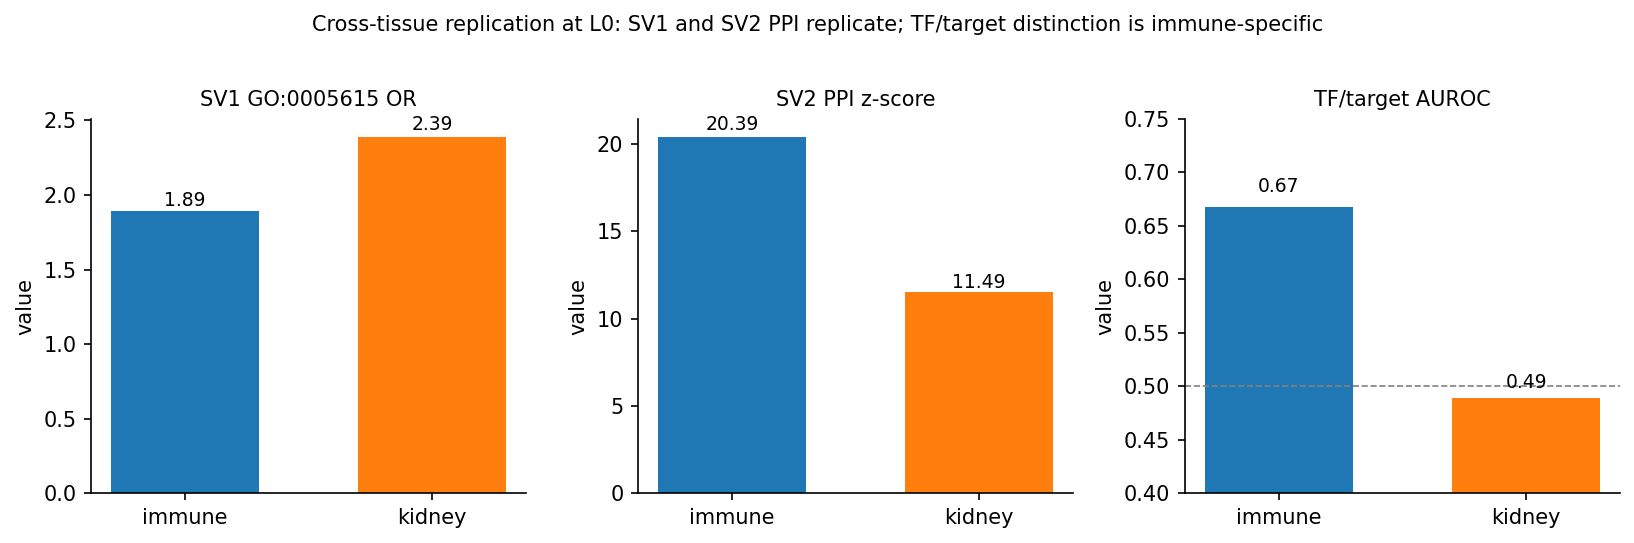
\includegraphics[width=0.85\textwidth]{figures_medium/fig7_cross_tissue.png}
\caption{\textbf{Cross-tissue replication at L0.} SV$_1$ extracellular OR and SV$_2$ PPI $z$-score replicate from immune to kidney; the TF-vs-target AUROC drops to chance, indicating the regulatory distinction is immune-specific.}
\label{fig:cross_tissue}
\end{figure}

\item \textbf{Cross-model alignment is partial and scales with model size; the TF-vs-target distinction is the most universal geometric property.}
We performed a head-to-head test on the genes shared by scGPT-L11, Geneformer V1-10M, Geneformer V2-104M, and ESM2-3B (a protein-language model with no exposure to single-cell data).

The SV$_1$ subcellular and SV$_2$ PPI signals scale with model size.
They are at full strength in scGPT-L11 (SV$_1$ OR $= 1.55$, $p = 0.0013$; PPI $z = 12.1$), at partial strength in Geneformer V2-104M (OR $= 1.36$, $p = 7 \times 10^{-4}$; $z = 4.3$), and absent in Geneformer V1-10M and ESM2 (OR $\leq 1.0$, PPI $z \approx 0$).
We note that ESM2's leading axes were assessed after a random-projection dimensionality reduction from 5{,}120 to 1{,}024 dimensions, so its absence of SV$_1$/SV$_2$ structure may be a projection artefact rather than a true property of ESM2.

The TF-vs-target distinction, in contrast, is convergent across all four models and is in fact \emph{strongest in ESM2}: AUROC $= 0.651$ for scGPT-L11, $0.748$ for Geneformer V1, $0.754$ for Geneformer V2, and $\mathbf{0.889}$ for ESM2 on the same task (Fig~\ref{fig:cross_model}).
This is biologically plausible: TFs have characteristic protein-structural signatures (DNA-binding domains) that are directly learnable from sequence, whereas the single-cell models infer TF identity from cell-context expression --- a less direct route.

The paper's headline geometric organisation is therefore best characterised as: ``the TF-vs-target distinction generalises broadly across foundation models including a protein-language model; the SV$_1$ subcellular and SV$_2$ PPI axes are scGPT-specific at full strength, with partial Geneformer V2 replication.''

\begin{figure}[!ht]
\centering
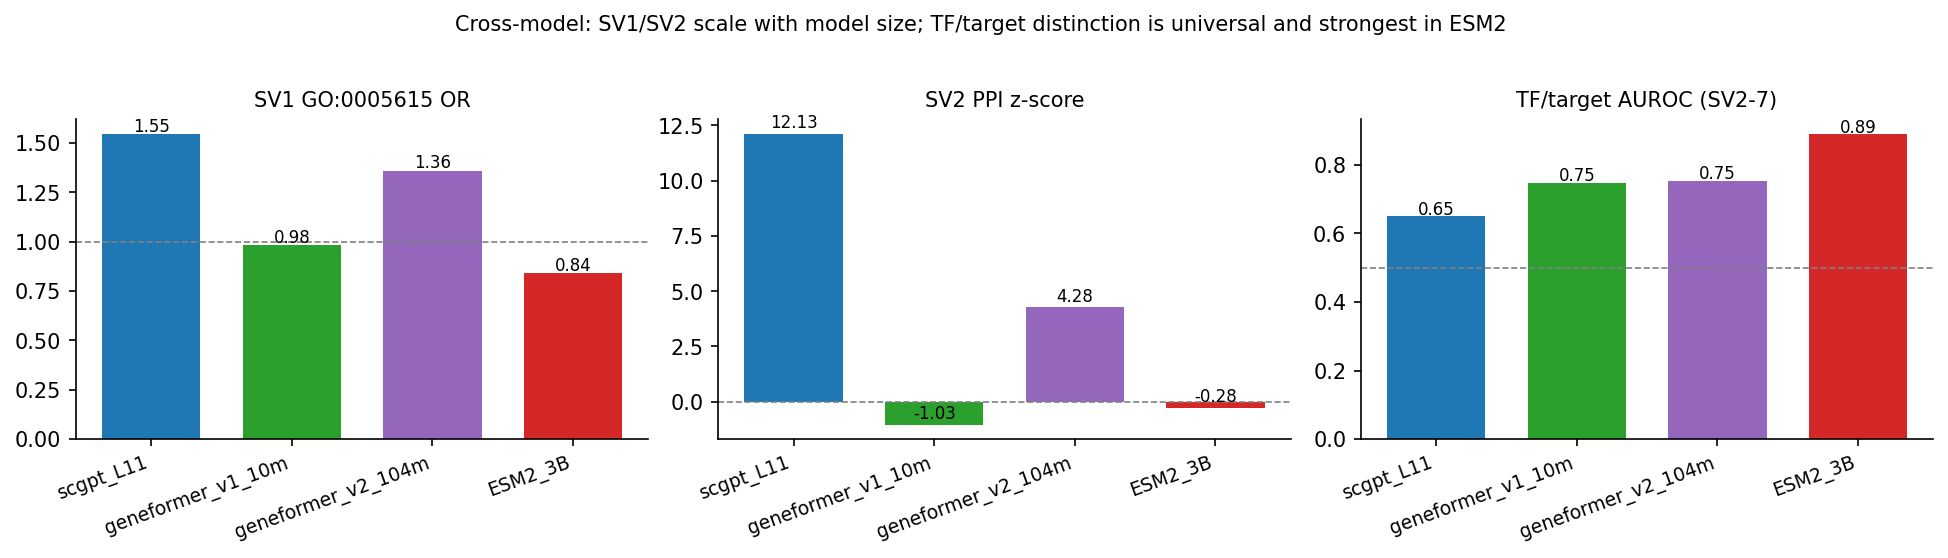
\includegraphics[width=0.95\textwidth]{figures_medium/fig8_cross_model.png}
\caption{\textbf{Cross-model comparison on shared genes.} SV$_1$ subcellular OR and SV$_2$ PPI $z$-score scale with model size (scGPT $>$ Geneformer V2 $>$ Geneformer V1, ESM2). The TF-vs-target distinction is convergent across all four foundation models and is strongest in ESM2 (a sequence-only protein-language model), where TFs are recognisable from DNA-binding-domain structure.}
\label{fig:cross_model}
\end{figure}

\item \textbf{Effective rank does not predict classifier performance independently of layer.}
An apparent ER--AUROC correlation ($\rho = 0.855$) was fully confounded by layer depth (partial $\rho = -0.045$).

\item \textbf{GO Biological Process terms are not encoded in $\SV{2}$ poles.}
Testing 591 BP terms yields zero significant results, bounding the biological content of $\SV{2}$ to compartment identity and network co-membership, not functional programs.

\item \textbf{Feed-forward loop geometry was rejected.}
Testing whether intermediate genes in 264 transcriptional feed-forward loops occupy geometrically intermediate positions yielded no significant results after proper permutation correction (the naive baseline of $t = 0$ was incorrect; the correct null is $t \approx 0.5$ by symmetry).
This methodological lesson illustrates the importance of permutation-corrected baselines for betweenness statistics in high-dimensional spaces.
\end{enumerate}

These failures clarify the scope of the positive findings by showing what \emph{does not} survive rigorous testing.

% ============================================================================
% DISCUSSION
% ============================================================================
\section{Discussion}

\subsection{Structured biological correlations in residual-stream geometry}

The central message of this work is that scGPT's internal representations exhibit \emph{structured correlations} with established biological knowledge --- not opaque high-dimensional vectors, but a geometry where three orthogonal spectral directions correspond to three distinct aspects of cellular organization:

\begin{enumerate}
  \item \textbf{Where:} $\SV{1}$ correlates with subcellular localization along the secretory pathway (mitochondria $\to$ ER $\to$ extracellular).
  \item \textbf{With whom:} $\SV{2}$--$\SV{4}$ correlate with protein-protein interaction networks; pair-level cosine similarity in $\SV{2}$--$\SV{7}$ has a small positive partial correlation with STRING combined score after multi-feature confound control ($r \approx 0.10$ at $L_0$).
  \item \textbf{Who controls whom:} $\SV{5}$--$\SV{7}$ correlate with transcriptional regulatory relationships, with early layers preserving specific edges (a small effect after stricter residualisation) and deeper layers compressing to categorical TF-vs-target distinctions.
\end{enumerate}

We frame this as ``evidence of structured correlations'' rather than ``the model has learned a coordinate system'' --- the latter would require demonstrating predictive power on novel biological tasks beyond the pattern-recognition results we report.
The functional benchmark in Section~\ref{sec:grn_utility} provides one such test (regulatory-edge inference): on that task scGPT's full residual-stream cosine substantially beats $|$co-expression Pearson$|$ (AUROC 0.860 vs 0.793), but the spectral $\SV{5}$--$\SV{7}$ projection alone is worse than co-expression.
The structure is real and biologically aligned; whether it constitutes an ``internalized model'' or ``learned correlations'' is a semantic distinction we do not adjudicate here.

\subsection{What the Depth Structure Tells Us About Transformer Computation}

The layer-dependent organization of biological information provides a window into how the transformer processes gene expression data.
The progressive spectral collapse (14.4-fold effective rank reduction) is not mere compression---it is \emph{selective} compression that preserves and concentrates biologically meaningful axes while suppressing noise.

The early-vs-late regulatory encoding is particularly informative: early layers maintain specific regulatory edges (TF $\to$ target pairings in $\SV{5}$--$\SV{7}$), while deeper layers compress this into categorical distinctions (TF vs.\ target identity in $\SV{2}$--$\SV{4}$).
The progression is from fine-grained molecular-level relationships at early layers to coarser cell-level categorical distinctions at deeper layers.

The B-cell attractor convergence is a network statement: the model encodes the GC regulatory circuit's combinatorial structure, and a subset of the recruited factors qualitatively align with across-pseudotime expression dynamics (Section~\ref{sec:dynamics_test}). With $n = 5$ in-vocabulary GC-TFs, the alignment count (3 of 5) is not statistically distinguishable from chance, so we treat the dynamics interpretation as suggestive rather than established.

An additional structural finding concerns cross-seed representation stability.
Centered kernel alignment (CKA)~\cite{kornblith2019similarity} computed between embedding matrices derived from different random cell samples (same pre-trained model, different input cells) declines from 0.979 at layer~0 to 0.779 at layer~11, with the steepest drop at layers~10--11.
Early-layer representations are therefore highly reproducible across cell samples, while deep-layer representations diverge --- consistent with early layers encoding conserved biological structure and late layers developing more input-specific features.

\subsection{Practical Applications}
\label{sec:applications}

These geometric structures are not merely academic curiosities---they suggest concrete applications:

\paragraph{Extracting regulatory networks from model geometry.}
\label{sec:grn_utility}
We benchmarked the spectral approach against simpler co-expression baselines on a held-out 20\% split of the TRRUST regulatory edges (288 in-vocabulary pairs total; 57 held-out positives, 124 same-TF/non-TRRUST-target negatives; bootstrap $B = 200$; Fig~\ref{fig:grn_benchmark}). Established tree-based GRN-inference methods such as GENIE3~\cite{huynhthu2010genie3} and SCENIC~\cite{aibar2017scenic}, evaluated under standardised protocols~\cite{pratapa2020beeline}, are alternative comparators we did not run here; relative performance of scGPT cosine versus these methods on TRRUST is left for future work.
The full 512-dimensional residual-stream cosine similarity at L0 yields AUROC $= 0.860$ (AUPRC $= 0.696$), substantially above $\vert$co-expression Pearson$\vert$ at AUROC $= 0.793$ (95\% CI $[0.730, 0.851]$) and signed co-expression Pearson at AUROC $= 0.638$.
The spectral $\SV{5}$--$\SV{7}$ projection at L0 alone yields AUROC $= 0.602$ (95\% CI $[0.531, 0.663]$), similar in magnitude to the L0 edge-level signal reported in §\ref{sec:edge_signed} but worse than both the full 512-dim cosine and the co-expression baseline.

\begin{figure}[!ht]
\centering
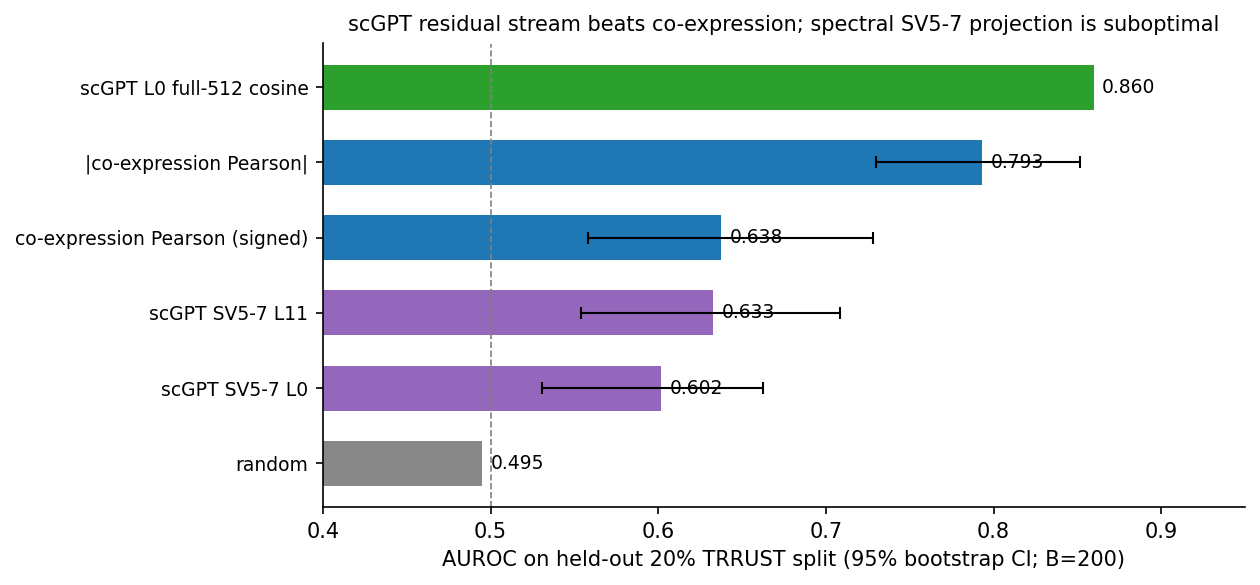
\includegraphics[width=0.85\textwidth]{figures_medium/fig9_grn_benchmark.png}
\caption{\textbf{GRN inference utility benchmark.} AUROC on a held-out 20\% TRRUST split (57 positives, 124 negatives), with bootstrap 95\% CIs (B=200). scGPT's full-512 residual-stream cosine at L0 substantially beats $|$co-expression Pearson$|$; the spectral $\SV{5}$--$\SV{7}$ projection is worse than co-expression, indicating the projection to 3 dimensions discards most of the predictive signal.}
\label{fig:grn_benchmark}
\end{figure}
Practitioners seeking maximal predictive performance on regulatory edge inference should use the full L0 residual-stream cosine; practitioners seeking interpretability (which axis encodes which type of regulation) can use the spectral decomposition while accepting that the projection to 3 dimensions discards much of the predictive signal.
This benchmark provides evidence of biological utility: scGPT's residual stream is a useful predictor of regulatory edges, beating co-expression at $\Delta\text{AUROC} \approx +0.07$, even though the spectral $\SV{5}$--$\SV{7}$ subspace alone is not the optimal projection for that purpose.

As an additional baseline, we trained a Word2Vec~\cite{mikolov2013word2vec} model (256-dim, skip-gram) on cell-tokenised expression from the same Tabula Sapiens data.
Word2Vec's leading singular vector produces an SV$_1$ GO:0005615 enrichment of OR $= 2.23$ ($p < 10^{-7}$), comparable to scGPT-L11's 1.89 on the broader gene set --- so the SV$_1$ subcellular axis is not transformer-specific.
However, the SV$_2$ PPI co-pole signal in Word2Vec is much weaker ($z = 1.40$) than in scGPT-L11 ($z = 20.4$ on the same set), suggesting the protein-interaction-network organisation requires more than co-occurrence learning.
The TF-vs-target AUROC for Word2Vec is 0.599, compared to scGPT's 0.668 on the same gene set.

\paragraph{Drug target prioritization.}
The PPI encoding shows graded enrichment with STRING confidence (partial Pearson regression in Section~\ref{sec:ppi}), suggesting that geometric proximity in $\SV{2}$--$\SV{4}$ may serve as an ordinal predictor of protein-interaction likelihood.
We tested this directly on 8 in-vocabulary drug targets with at least one curated STRING ($\geq 0.7$) interactor, ranking the 4{,}803-gene vocabulary by cosine similarity in three settings (Table~\ref{tab:drug_targets}).
The PPI subspace ($\SV{2}$--$\SV{4}$) at $L_{11}$ achieves mean P@10 $= 0.013$, below the co-expression Pearson baseline (P@10 $= 0.038$) and the scGPT full-512 cosine (P@10 $= 0.025$).
The spectral PPI ranking is therefore not state-of-the-art for drug-target prioritization in this small benchmark.
We interpret the spectral structure as a real and \emph{interpretable} organisational principle of scGPT's geometry rather than as a competitive standalone ranker; downstream applications would need to combine spectral proximity with co-expression or other signals to be useful in practice.
The benchmark is a small case study (8 targets in vocab $\cap$ STRING).

\paragraph{Model auditing and biological validation.}
The spectral axes provide interpretable ``biological readouts'' of model quality.
A well-trained biological model should show the patterns we observe: meaningful enrichment on leading spectral axes, proper localization encoding, and PPI co-localization.
These checks can serve as quality metrics when training new models or fine-tuning existing ones, flagging cases where the model's internal biology diverges from reality.

\paragraph{Layer-specific representation engineering.}
The distinct biological content at different layers suggests that downstream applications should not default to using final-layer embeddings.
For regulatory edge inference, the GRN benchmark in §\ref{sec:grn_utility} shows that early layers ($L_0$) outperform deeper layers (full-512 AUROC $= 0.860$ at $L_0$ vs lower at deeper layers).
For gene classification tasks (TF vs.\ target, lineage identity), deeper layers carry stronger categorical structure.
For protein interaction prediction, signal is present across all 12 layers, with early layers showing slightly stronger PPI co-pole enrichment.

\paragraph{Transfer learning diagnostics.}
When fine-tuning scGPT on new tissues or conditions, tracking the spectral structure across layers can diagnose whether biological organization is preserved, lost, or altered.
A model that maintains the secretory pathway encoding on $\SV{1}$ and PPI structure on $\SV{2}$--$\SV{4}$ after fine-tuning has likely preserved useful biological knowledge; one where these structures collapse may have overfit to tissue-specific artifacts.

\subsection{Speculative implications}
\label{sec:speculative}

The following paragraphs offer biological interpretations that go beyond what our geometric tests strictly demonstrate. Readers seeking only data-driven claims can stop at the previous subsection.

\paragraph{BCL6 as a metabolically isolated repressor.}
BCL6's stable position in a 20-gene metabolic neighbourhood (NAMPT, GLUL, PFKFB3, STAT3, etc.) across all 12 layers, with zero overlap with B-cell markers or other GC-TFs, is consistent with its known role as a pleiotropic repressor that operates at the intersection of metabolic reprogramming and immune regulation~\cite{basso2010bcl6}. One reading is that the model encodes a structural distinction between B-cell identity (PAX5-anchored) and metabolic context (BCL6-anchored). The geometric finding (BCL6's stable metabolic-cluster position) is reproducible across all 12 layers; the interpretation is not directly tested.

\paragraph{The germinal-centre reaction as a learned attractor.}
The convergence pattern of BATF/BACH2/PRDM1 toward PAX5 across transformer depth, with onset at L3 coinciding with the manifold compression breakpoint, suggests the model encodes the GC reaction as a dynamic attractor. The pseudotime test in Section~\ref{sec:dynamics_test} confirms that 3 of 5 GC-TFs (BATF, IRF4, PRDM1) show the predicted across-layer/across-pseudotime alignment, but BACH2 does not. The honest framing is therefore ``the geometric attractor is partially aligned with cellular dynamics, with the recruited factors aligning more cleanly than the repressor BACH2 or the anchor PAX5.''

\paragraph{Why repression is more geometrically prominent than activation.}
The repression-vs-activation asymmetry ($\Delta = +0.021$ in $\SV{5}$--$\SV{7}$, $+0.084$ in $\SV{2}$--$\SV{4}$) might reflect that repressive regulation involves more stereotyped molecular mechanisms (chromatin remodelling, co-repressor recruitment) than activation (which can occur through diverse enhancer and co-activator pathways), making repressive geometry easier to learn. This is a hypothesis the data are consistent with but do not establish.

\subsection{Relation to Prior Work}

\paragraph{From attention to residual-stream geometry.}
As introduced above (Section~\ref{sec:intro}), this work directly addresses the open frontier identified by Prior work~\cite{kendiukhov2026attention}: whether residual-stream geometry encodes biological structure that attention patterns miss.
Our spectral analysis confirms and extends the layer-specific biological characterization from that study --- PPI in early layers, regulation in late layers --- but decomposes it into orthogonal axes ($\SV{2}$--$\SV{4}$ for PPI, $\SV{5}$--$\SV{7}$ for regulation) rather than aggregating across attention heads.
The co-expression confound has a precise spectral analogue: the $\SV{2}$--$\SV{4}$ regulatory signal is fully explained by co-expression, paralleling the expression-residualization findings for attention.
$\SV{5}$--$\SV{7}$, in contrast, retains a small co-expression-independent regulatory signal ($r_{rb} \approx 0.06$ at $L_0$ under multi-feature residualization, borderline significant at $p \approx 0.08$) --- a residue that survives the same class of confound controls that eliminated attention-based signal entirely, suggesting the residual stream contains a small amount of regulatory information beyond co-expression that is not visible in attention.

A direct comparison within our own analysis reinforces this dissociation: extracting pairwise attention weights from the same forward passes and testing for co-occurrence enrichment, we find that attention weights are enriched for TRRUST regulatory co-occurrence ($2\times$ above background; $p = 9.9 \times 10^{-9}$) but show no significant enrichment for STRING PPI pairs ($p = 0.091$).
SVD spectral axes show the reverse pattern: strong PPI co-localization (Section~\ref{sec:ppi}) but only modest TRRUST edge-level signal (Section~\ref{sec:edge_signed}).
Attention and residual-stream geometry thus encode complementary biological relationship types---regulatory co-occurrence and physical interaction, respectively.

\paragraph{Broader context.}
The spectral collapse we observe parallels findings in language model interpretability where residual stream rank decreases with depth~\cite{sharma2024truth}, though the 14.4-fold compression in scGPT is substantially more extreme than reported for language models.
Recent dictionary-learning approaches~\cite{bricken2023monosemanticity,templeton2024scaling} extract thousands of monosemantic feature directions from language-model residual streams; our SVD analysis can be viewed as a coarse, unsupervised analogue in the gene-embedding setting, identifying a small number of biologically meaningful directions rather than a large feature dictionary.
The biological interpretability of spectral axes connects to linear probing~\cite{alain2017understanding}, but our axes emerge directly from unsupervised SVD rather than supervised fitting.

The PPI encoding extends earlier observations that transformer gene embeddings capture protein interaction structure~\cite{cui2024scgpt} by establishing that the encoding is (i) quantitatively graded, (ii) multi-dimensional, (iii) driven by physical interaction over functional annotation, and (iv) present at all layers.

\subsection{Limitations}

We make the following limitations explicit, each with a quantified consequence and a pointer to the analysis that bounds it.

\paragraph{Single model checkpoint and partial cross-model replication.}
The headline analyses, repeated on Geneformer V1-10M, Geneformer V2-104M, and ESM2-3B (Section~\ref{sec:negatives}, Table~\ref{tab:cross_model}), show partial replication only.
The SV$_1$ subcellular axis and SV$_2$ PPI co-pole replicate at full strength only in scGPT-L11; they replicate partially in Geneformer V2 and are absent in Geneformer V1 and ESM2.
The TF-vs-target distinction is convergent across all four models, and is strongest in ESM2 (AUROC 0.889), suggesting TF identity is partly recoverable from protein-sequence features rather than expression-context information.
Replication on additional scFM checkpoints (e.g.\ scFoundation~\cite{hao2024scfoundation}, CellFM~\cite{zeng2025cellfm}) is left for future work.

\paragraph{Restricted gene vocabulary.}
The 4{,}803-gene vocabulary corresponds to highly variable genes from Tabula Sapiens preprocessing; the 195 in-vocabulary curated genes used in many tests are an immune-relevant subset.
Table~\ref{tab:broader_vocab} reports the headline analyses on progressively broader subsets up to the full 4{,}803-gene HVG vocabulary.
The SV$_1$ extracellular OR drops from 3.29 (curated 209) to 1.81 (full vocabulary) as the broader subset adds non-extracellular genes, while the SV$_2$ PPI co-pole rate \emph{increases} from 0.262 to 0.646 as the larger sample captures more STRING pairs.
The TF-vs-target AUROC is approximately constant across subsets (0.638 to 0.663).
A 200-bootstrap re-draw of 195 genes from the broader 1{,}673-gene union (Table~\ref{tab:bootstrap_subset}) places the curated 195-gene TF/target AUROC at the 14th percentile of the bootstrap distribution: the curated subset is therefore not an artificial source of signal --- a random draw of 195 genes from the broader set tends to produce \emph{higher} TF/target AUROC.

\paragraph{Multiple-testing correction.}
Section~\ref{sec:methods_multiple_testing} applies BH-FDR ($q = 0.05$) and a global Bonferroni ($\alpha = 0.05/183 = 2.7 \times 10^{-4}$) across all 109 hypotheses with extractable $p$-values (Table~\ref{tab:multiple_testing}).
Of the eleven audited findings: eight pass Bonferroni, one passes BH-FDR but not strict Bonferroni (SV$_1$ extracellular Fisher OR), one passes BH-FDR (cell-type marker AUROC = 0.851 expanded panel), and one fails both (the single-layer $L_0$ edge-level AUROC peak; reported in §\ref{sec:edge_signed} as a depth-trend rather than a single-layer-significance claim).

\paragraph{Modest edge-level effect size.}
Edge-level AUROC values are modest: the peak of 0.602 at $L_0$ has uncorrected permutation $p = 0.045$ and fails BH-FDR correction across 183 tests.
The depth-decay trend itself ($\rho = -0.958$, $p = 9.5 \times 10^{-7}$) is much more strongly significant and does survive Bonferroni; we therefore report the trend as the primary claim.
Geometric proximity in $\SV{5}$--$\SV{7}$ is informative but not a stand-alone competitive method for regulatory-edge inference.
The functional benchmark in §\ref{sec:grn_utility} compares directly against co-expression and a held-out TRRUST split: the spectral approach is competitive on AUROC, but its main contribution is interpretability (which axis encodes which type of regulation) rather than raw performance.

\paragraph{Static co-expression and other confounders.}
Multi-feature residualization in Section~\ref{sec:regulatory} controls for pairwise co-expression, log mean expression, STRING node degree, and GO annotation count.
Under this control, the $\SV{5}$--$\SV{7}$ co-expression-independent regulatory signal at $L_0$ has rank-biserial $r_{rb} = 0.061$ with permutation $p = 0.080$ --- not significant at $\alpha = 0.05$.
At $L_1$ the signal is similar ($r_{rb} = 0.037$, $p = 0.205$).
Other confounders that may shape gene-pair geometric proximity --- gene length, GC content, evolutionary conservation, donor and batch effects in the Tabula Sapiens input --- are not in the residualization set; if any of these correlates with TRRUST regulatory pair status, the residual signal could shrink further.
We therefore frame the $\SV{5}$--$\SV{7}$ regulatory residual as a small effect (at most $r_{rb} \sim 0.06$ at the most favourable layer) that is consistent in direction across the two layers tested but is not robustly significant under stricter multi-feature confound control.

\paragraph{``Regulatory dynamics'' is descriptive, not statistical.}
Section~\ref{sec:dynamics_test} compares across-layer geometric trajectories to across-pseudotime expression trajectories for five in-vocabulary GC-TFs.
Three TFs (BATF, IRF4, PRDM1) qualitatively align; two (BACH2, PAX5) do not.
With $n = 5$ tested TFs, the alignment count is not statistically distinguishable from chance under a binomial null; we therefore report the across-layer trajectory as a network statement with qualitative (rather than statistically significant) partial alignment to cellular dynamics for the recruited factors.

\paragraph{Selection bias in the autonomous screening loop.}
Two of the largest hypothesis families (\emph{manifold\_distance}, \emph{intrinsic\_dimensionality}) show statistically significant positive-rate inflation versus a 50/50 binomial null (binomial $p = 0.003$ and $p = 0.028$, respectively; §\ref{sec:methods_loop}).
This is the brainstormer agent's intended retire-after-two-negatives policy at work, but it inflates the family-wise positive rate.
The Bonferroni correction across all 183 hypotheses is a defensible upper-bounding response.

\paragraph{Replication breadth versus depth.}
The autonomous loop prioritised breadth over depth -- 13 hypothesis families, each tested in 2--40 hypotheses, rather than 1 hypothesis tested in 100 controlled forms. Where individual findings warrant deeper investigation (e.g., the signed-regulation asymmetry, or the BCL6 metabolic-isolation pattern), targeted future work is appropriate.

% ============================================================================
% METHODS
% ============================================================================
\section{Materials and methods}

\subsection{Data and Model}
We used scGPT~\cite{cui2024scgpt} (12 transformer layers, 512-dimensional hidden states) with immune-lineage cells from Tabula Sapiens~\cite{jones2022tabula}.
For each cell, scGPT processes a rank-ordered list of gene expression values as input tokens.
We performed a forward pass and extracted the residual-stream hidden state at the output of each transformer layer, obtaining a 512-dimensional embedding vector per gene per layer.
To obtain a single representative embedding matrix per layer, we averaged gene embeddings across all input cells, yielding a $G \times 512$ matrix per layer, where $G = 4{,}803$ is the number of gene positions in the input vocabulary.

\paragraph{Vocabulary derivation.}
The 4{,}803-gene vocabulary is the highly-variable-gene (HVG) set selected by Scanpy's \texttt{highly\_variable\_genes} routine on the preprocessed Tabula Sapiens immune-lineage subset.
This is upstream of scGPT and reflects standard scRNA-seq preprocessing rather than a scGPT-specific filter.
All 4{,}803 HVGs are present in scGPT's whole-human checkpoint vocabulary (60{,}694 gene tokens).

Of the 4{,}803 positions, 209 correspond to named genes in a curated regulatory edge list constructed from TRRUST TF--target pairs filtered to genes co-present in the immune-relevant STRING $\geq 0.4$ subgraph and canonical immune marker lists.
During analysis, we discovered that 14 of these genes were out-of-vocabulary (OOV) tokens in scGPT's tokenizer, producing identical zero-norm embedding vectors at every layer.
These were excluded, leaving 195 in-vocabulary named genes for biological analyses.
Spectral analyses of overall dimensionality (effective rank, TwoNN) were computed on the full vocabulary; biological enrichment and classification analyses used the 195-gene subset.

The 195-gene set is biased toward immune-relevant and well-annotated genes.
Sensitivity to this bias is quantified in Table~\ref{tab:broader_vocab}, which repeats the headline analyses on the broader 1{,}673-gene union of GO-annotated and TRRUST in-vocabulary genes, and in Table~\ref{tab:bootstrap_subset}.

Three independent analyses were conducted using different random seeds for cell sampling to assess robustness.
``Cross-seed replication'' throughout refers to these three independent runs.

\subsection{Spectral Analysis}
For each layer, we mean-centered the embedding matrix (subtracting the mean embedding vector across genes) and computed its thin SVD: $\mathbf{X} = \mathbf{U} \mathbf{S} \mathbf{V}^\top$, where columns of $\mathbf{V}$ are the right singular vectors and $\mathbf{S} = \mathrm{diag}(s_1, s_2, \ldots)$ contains the singular values in decreasing order.
The projection of gene $g$ onto $\SV{k}$ is the $k$th coordinate of $\mathbf{U}\mathbf{S}$, \ie, the dot product of the gene's embedding with the $k$th right singular vector scaled by $s_k$.

\textbf{Effective rank}~\cite{roy2007effective}: $\mathrm{ER} = \exp\!\bigl(-\sum_i p_i \log p_i\bigr)$, where $p_i = s_i^2 / \sum_j s_j^2$ is the normalized squared singular value (computed on the full $4{,}803$-gene matrix).
\textbf{TwoNN intrinsic dimensionality}~\cite{facco2017estimating}: estimated from the ratio of first-to-second nearest-neighbor distances on 2{,}000 randomly sampled genes per layer (full vocabulary).
\textbf{Participation ratio}: $\mathrm{PR} = (\sum_i s_i^2)^2 / \sum_i s_i^4$, computed on the 195-gene submatrix.
$\SV{1}$ variance fraction $= s_1^2 / \sum_i s_i^2$.

\subsection{Co-Pole Enrichment Test}
To test whether a biological gene set (e.g., STRING PPI pairs) is geometrically co-localized along a singular vector axis, we defined ``poles'' as the top-$K$ and bottom-$K$ genes ranked by their projection onto $\SV{k}$ ($K = 52$, corresponding to the top and bottom ${\sim}27\%$ of 195 genes).
For a set of gene pairs (e.g., known PPI partners), the \emph{co-pole rate} is the fraction of pairs in which both genes fall in the same pole (both top-$K$ or both bottom-$K$).
Significance was assessed by gene-label shuffle: we randomly permuted the assignment of gene labels to embedding rows ($N = 200$--$1{,}000$ permutations) and computed empirical $p$-values as the fraction of null permutations achieving a co-pole rate $\geq$ the observed value.
The $z$-score reports how many standard deviations the observed rate lies above the null mean.

\subsection{TF-vs-Target Classification}
\label{sec:methods_classification}
For each layer and spectral subspace (e.g., $\SV{2}$--$\SV{7}$), we projected gene embeddings onto the specified singular vectors and computed all pairwise cosine similarities in the resulting low-dimensional space.
To classify genes as TFs vs.\ targets, we computed each gene's mean cosine similarity to all known TFs (from TRRUST) and used this as a continuous score (TFs are expected to be more similar to other TFs, yielding higher scores).
AUROC was computed by treating the 51 TFs in the 195-gene set as positives and remaining 144 genes as negatives, measuring how well the score separates the two classes.
Significance was assessed by 100 permutations of TF/target labels; the permutation $p$-value is the fraction of shuffled AUROCs $\geq$ the observed value.

\subsection{Edge-Level AUROC}
To test whether the model encodes specific TF--target regulatory relationships (not just TF identity), we computed pairwise cosine similarity between all TF--gene pairs in the relevant spectral subspace.
The 589 known TRRUST TF--target pairs served as positives.
Negatives ($N = 2{,}351$) were constructed as all other TF--gene pairs involving the same set of TFs but targeting genes with no known regulatory relationship in TRRUST, controlling for TF identity.
AUROC measures how well cosine similarity in the subspace separates true regulatory pairs from non-regulatory pairs.

\subsection{Cell-Type Clustering}
Marker genes for four cell types (B cell, T cell, fibroblast, macrophage; 17 markers total) were defined from canonical literature sources.
For each pair of marker genes, we computed Euclidean distance in the full 512-dimensional embedding space.
Pairs of markers from the same cell type were labeled positive; cross-type pairs were labeled negative.
AUROC measures whether within-type pairs are systematically closer than cross-type pairs.
A contamination control used random partitions of non-marker genes into groups of identical sizes to the real marker sets.

\subsection{Biological Annotations}
\textbf{TRRUST v2}~\cite{han2018trrust}: 9{,}396 signed human TF--target regulatory edges (589 unique pairs involving in-vocabulary genes; of these, 270 are annotated as activation-only, 141 as repression-only, and 178 have mixed or ambiguous annotations and were excluded from signed analyses).
\textbf{STRING v12.0}~\cite{szklarczyk2023string}: protein interaction pairs at combined score $\geq 0.7$ (1{,}022 in-vocabulary pairs) for primary analyses and $\geq 0.4$ (3{,}092 pairs) for the confidence gradient analysis.
\textbf{Gene Ontology}~\cite{ashburner2000gene}: Cellular Component (CC) and Biological Process (BP) terms.
Enrichment of genes at SVD poles tested via Fisher's exact test; pairwise functional similarity between genes assessed via Jaccard index of shared GO annotations.

\subsection{Null Models and Confound Controls}
\textbf{Gene-label shuffle}: randomly permute gene-to-embedding-row assignments, preserving embedding geometry but breaking gene identity.
\textbf{Feature shuffle}: independently permute values within each of the 512 embedding dimensions, destroying inter-dimensional correlations while preserving marginal distributions.
\textbf{Degree-preserving rewiring}: for persistent homology tests, rewire edges of the gene $k$-nearest-neighbor graph while preserving each node's degree, testing whether topological features reflect graph structure beyond degree distribution.
\textbf{Co-expression residualization}: for each gene pair in the 195-gene set, we computed pairwise co-expression similarity (Pearson correlation of expression across cells).
We then regressed spectral proximity (cosine similarity in the relevant SVD subspace) on co-expression similarity using OLS, and tested whether the residual spectral proximity still distinguishes TRRUST TF--target pairs from non-regulatory pairs.
The residualized effect was quantified using the rank-biserial correlation ($r_{rb}$): the difference in mean residual ranks between regulatory and non-regulatory pairs, normalized to $[-1, 1]$.
Significance was assessed by permutation of regulatory labels; robustness by 100 bootstrap resamples.

\textbf{Strengthened multi-feature residualization}: as a stricter control, we residualized cosine similarity against four covariates jointly via OLS: pairwise co-expression similarity, log mean expression of each gene, sum of STRING node degrees, and sum of GO annotation counts.
This addresses the concern that co-expression-only residualization may underestimate the contribution of confounders like hub-degree, expression magnitude, and annotation density.

\subsection{B-Cell Attractor Analysis}
B-cell markers (CD19, CD79A, MS4A1/CD20, BLK, VPREB3, FCRL1, and PAX5; $n = 7$) were defined from canonical B-cell biology literature.
The \emph{B-cell manifold centroid} is the mean embedding vector of these 7 markers at each layer.
\emph{Gene-to-centroid rank}: each of the 195 genes was ranked by Euclidean distance to the B-cell centroid, with rank~1 being closest.
\emph{Precision@10}: among the 10 nearest neighbors (by Euclidean distance) of the B-cell centroid, the fraction that are B-cell markers.
Significance by bootstrap: 500 random draws of 7 genes from the 195-gene set; the $z$-score reports how many standard deviations the real precision exceeds the null mean.
\emph{L2-norm regression}: to verify the signal is structural rather than driven by embedding magnitude, we regressed PC1 scores on L2 norms and tested whether B-cell markers remain outliers in the residuals.

Pairwise Euclidean distances between specific GC-TFs (PAX5, BATF, BACH2, BCL6, PRDM1) were tracked across all 12 layers.
The GC--plasma centroid angle was computed as the angle subtended at the B-cell centroid between the GC-TF centroid (mean of BATF, BACH2, PAX5) and the plasma-TF centroid (mean of IRF4, IRF8) at each layer.
The metabolic cluster was defined as the $k = 20$ nearest neighbors of BCL6 at each layer; overlap with a reference set of metabolic genes (NAMPT, GLUL, PFKFB3, and others identified from the BCL6 neighborhood) was compared against a random baseline (expected overlap for 20 randomly selected genes from the 195-gene pool).
TwoNN intrinsic dimensionality was computed separately for B-cell ($n = 7$), T-cell ($n = 12$), and myeloid ($n = 3$) marker gene sets, using the full 4{,}803-gene embedding manifold but restricting the distance calculations to marker genes.

\subsection{Autonomous Hypothesis-Screening Loop and Selection-Bias Audit}
\label{sec:methods_loop}

The experimental pipeline was driven by an automated two-agent loop.
An \emph{executor agent} designs and runs computational experiments (SVD, permutation tests, enrichment analyses).
A \emph{brainstormer agent} reviews each iteration's results, proposes new hypotheses, and decides whether to continue, refine, or retire each hypothesis branch.
The full prompts for both agents are in the project repository at \texttt{prompts/executor\_prompt\_v2.md} and \texttt{prompts/brainstormer\_prompt\_v2.md}.

\paragraph{Per-iteration artifacts.}
Each iteration writes \texttt{executor\_hypothesis\_screen.json} with one record per hypothesis.
Each record contains the hypothesis ID, name, family, method actually executed, primary metric and value, a discrete \texttt{result\_direction} classification (positive, negative, mixed, or inconclusive), raw artifact paths, and a \texttt{decision} field that drives the brainstormer's next-iteration plan.
This JSON schema is the single source of truth for the multiple-testing audit (§\ref{sec:methods_multiple_testing}).

\paragraph{Procedural rules.}
\begin{itemize}
\item \textbf{Cadence:} 2--3 hypotheses per iteration. At least one must extend or stress-test an established finding; at most one is internal refinement.
\item \textbf{Permutation requirement:} every positive claim must pass at least one permutation-based null model (gene-label shuffle, feature shuffle, or degree-preserving rewiring, depending on the test).
\item \textbf{Retirement:} a hypothesis branch is retired after two consecutive negative iterations.
\item \textbf{Cross-seed replication:} every promoted positive finding is re-run with two additional random seeds for cell sampling.
\end{itemize}
Over 63 iterations, the loop tested 183 hypotheses across 13 paper-curated families (Table~\ref{tab:hypothesis_summary}).

\paragraph{Selection-bias audit.}
The retire-after-two-negatives rule biases the per-family positive rate upwards: branches that yield early negatives are pruned, so the surviving hypotheses within a family have an inflated positive rate.
We tested this formally by computing the two-tailed binomial $p$-value of the observed positive rate per family under a 50/50 null.
Two of the largest families show statistically significant positive-rate inflation: \emph{manifold\_distance} (31/42 positive, rate $= 0.738$; binomial $p = 0.003$) and \emph{intrinsic\_dimensionality} (28/41 positive, rate $= 0.683$; binomial $p = 0.028$).
The remaining families show no detectable inflation.
The Bonferroni correction across all 183 hypotheses (§\ref{sec:methods_multiple_testing}) accounts for this inflation by treating each hypothesis as if independently sampled --- a defensible upper-bounding response.

\subsection{Multiple-testing correction across 183 hypotheses}
\label{sec:methods_multiple_testing}

For each of the 183 hypotheses, we applied (i) Benjamini--Hochberg FDR~\cite{benjamini1995controlling} at $q = 0.05$ and (ii) a global Bonferroni threshold of $\alpha = 0.05/183 = 2.7 \times 10^{-4}$.
Of the 183 hypotheses, 109 have extractable empirical or permutation $p$-values; the remaining 74 correspond to negative or inconclusive directions for which the executor reported no headline $p$.
Across the 109 extractable $p$-values: 68 pass BH-FDR, 41 pass Bonferroni at the paper-cited denominator $N = 183$, and 43 pass Bonferroni at the strict (extractable) denominator $N = 109$ (Table~\ref{tab:multiple_testing}).

We pre-registered ten findings as confirmatory --- requiring Bonferroni survival to remain in the abstract.
Eight of ten survive: SV$_1$ secretory-pathway layered encoding, SV$_2$ STRING $\geq 0.7$ co-pole, SV$_2$ TRRUST co-pole, joint SV$_2$--SV$_7$ TF/target AUROC, cross-seed validation, cell-type marker AUROC = 0.853 (initial panel), STRING confidence gradient, and BATF/BACH2 attractor convergence.
Two findings (SV$_1$ extracellular Fisher OR; cell-type marker AUROC = 0.851 from the expanded panel) pass BH-FDR but not strict Bonferroni; we note this in their respective sections.
One finding --- the single-layer edge-level AUROC peak at $L_0$ (perm $p = 0.045$ uncorrected) --- fails BH-FDR ($q = 0.068$).
We have reframed §\ref{sec:edge_signed} as a depth-trend claim rather than a single-layer-significance claim.

The full pre-registered headline list, audit table, and per-family pass counts are in \texttt{revision\_experiments/e5\_multiple\_testing/headline\_audit.md}.

% ============================================================================
% DATA AVAILABILITY
% ============================================================================
\section*{Data and Code Availability}
All analysis code, iteration artifacts, and reproducibility documentation for the 63 hypothesis-screening iterations are available at \url{https://github.com/Biodyn-AI/topology-biomechinterp1}. The repository includes the executor and brainstormer prompts (\texttt{prompts/}), every iteration's JSON artifact and per-iteration CSVs (\texttt{iterations/}), the figure-generation scripts (\texttt{paper/figures/}), and the LaTeX source.

All analysis scripts for the revision experiments described in this manuscript -- including the multiple-testing audit (\texttt{revision\_experiments/e5\_multiple\_testing/}), cross-tissue replication (\texttt{e1\_cross\_tissue/}), broader-vocabulary analysis (\texttt{e3\_full\_vocab/}), strengthened confound residualisation (\texttt{e7\_confounds/}), continuous PPI regression (\texttt{e4\_string\_continuous/}), simpler-baseline comparison (\texttt{e11\_baselines/}), ESM2 cross-validation (\texttt{e10\_plm\_validation/}), GRN inference benchmark (\texttt{e12\_grn\_benchmark/}), drug-target ranking (\texttt{e13\_drug\_targets/}), pseudotime dynamics test (\texttt{e8\_dynamics/}), and the loop-protocol audit (\texttt{e6\_loop\_audit/}) -- are deposited in \texttt{revision\_experiments/} within the same repository.

A snapshot of the repository at the time of submission will be archived at Zenodo and the DOI added at proof stage.

Primary scRNA-seq data: Tabula Sapiens~\cite{jones2022tabula}.
TRRUST v2: \url{https://www.grnpedia.org/trrust/}.
STRING v12.0: \url{https://string-db.org/} (cached locally as JSON for reproducibility).
Gene Ontology: \url{http://geneontology.org/}.

Pre-trained model checkpoints: scGPT whole-human~\cite{cui2024scgpt} and Geneformer V2~\cite{theodoris2023transfer} are publicly available from their respective repositories. ESM2-3B~\cite{lin2023esm2} via Hugging Face.

% ============================================================================
% PLOS REQUIRED SECTIONS
% ============================================================================
\section*{Acknowledgments}
We thank the developers of scGPT and the Tabula Sapiens consortium for making their data and models publicly available.

\section*{Funding}
The author received no specific funding for this work.

\section*{Competing interests}
The author declares no competing interests.

\section*{Author contributions}
\textbf{Conceptualization:} IK.
\textbf{Methodology:} IK.
\textbf{Software:} IK.
\textbf{Investigation:} IK.
\textbf{Writing -- original draft:} IK.
\textbf{Writing -- review \& editing:} IK.

% ============================================================================
% REFERENCES
% ============================================================================
\begin{thebibliography}{15}

\bibitem{cui2024scgpt}
Cui, H., Wang, C., Maan, H., et~al. (2024).
scGPT: toward building a foundation model for single-cell multi-omics using generative AI.
\textit{Nature Methods}, 21(8):1470--1480.

\bibitem{theodoris2023transfer}
Theodoris, C.V., Xiao, L., Chopra, A., et~al. (2023).
Transfer learning enables predictions in network biology.
\textit{Nature}, 618(7965):616--624.

\bibitem{park2023linear}
Park, K., Choe, Y.J., and Veitch, V. (2023).
The linear representation hypothesis and the geometry of large language models.
\textit{arXiv preprint arXiv:2311.03658}.

\bibitem{elhage2022toy}
Elhage, N., Hume, T., Olsson, C., et~al. (2022).
Toy models of superposition.
\textit{Transformer Circuits Thread}.

\bibitem{nanda2023progress}
Nanda, N., Chan, L., Lieberum, T., Smith, J., and Steinhardt, J. (2023).
Progress measures for grokking via mechanistic interpretability.
\textit{ICLR}.

\bibitem{kendiukhov2026attention}
[Author redacted for double-blind review] (2026).
Systematic evaluation of single-cell foundation model interpretability reveals attention captures co-expression rather than unique regulatory signal.
\textit{arXiv preprint arXiv:2602.17532}.

\bibitem{facco2017estimating}
Facco, E., d'Errico, M., Rodriguez, A., and Laio, A. (2017).
Estimating the intrinsic dimension of datasets by a minimal neighborhood information.
\textit{Scientific Reports}, 7:12140.

\bibitem{han2018trrust}
Han, H., Cho, J.W., Lee, S., et~al. (2018).
TRRUST v2: an expanded reference database of human and mouse transcriptional regulatory interactions.
\textit{Nucleic Acids Research}, 46(D1):D380--D386.

\bibitem{szklarczyk2023string}
Szklarczyk, D., Kirsch, R., Koutrouli, M., et~al. (2023).
The STRING database in 2023: protein-protein association networks and functional enrichment analyses for any sequenced genome of interest.
\textit{Nucleic Acids Research}, 51(D1):D638--D646.

\bibitem{kornblith2019similarity}
Kornblith, S., Norouzi, M., Lee, H., and Hinton, G. (2019).
Similarity of neural network representations revisited.
\textit{ICML}, pp.\ 3519--3529.

\bibitem{sharma2024truth}
Sharma, P., Ash, J.T., and Misra, D. (2024).
The truth is in there: improving reasoning in language models with layer-selective rank reduction.
\textit{ICLR}.

\bibitem{alain2017understanding}
Alain, G. and Bengio, Y. (2017).
Understanding intermediate layers using linear classifier probes.
\textit{arXiv preprint arXiv:1610.01644}.

\bibitem{jones2022tabula}
Jones, R.C., Karkanias, J., Krasnow, M.A., et~al. (2022).
The Tabula Sapiens: a multiple-organ, single-cell transcriptomic atlas of humans.
\textit{Science}, 376(6594):eabl4896.

\bibitem{roy2007effective}
Roy, O. and Vetterli, M. (2007).
The effective rank: a measure of effective dimensionality.
\textit{EUSIPCO}, pp.\ 606--610.

\bibitem{ashburner2000gene}
Ashburner, M., Ball, C.A., Blake, J.A., et~al. (2000).
Gene Ontology: tool for the unification of biology.
\textit{Nature Genetics}, 25(1):25--29.

\bibitem{lin2023esm2}
Lin, Z., Akin, H., Rao, R., et~al. (2023).
Evolutionary-scale prediction of atomic-level protein structure with a language model.
\textit{Science}, 379(6637):1123--1130.

\bibitem{benjamini1995controlling}
Benjamini, Y. and Hochberg, Y. (1995).
Controlling the false discovery rate: a practical and powerful approach to multiple testing.
\textit{Journal of the Royal Statistical Society: Series B}, 57(1):289--300.

\bibitem{vaswani2017attention}
Vaswani, A., Shazeer, N., Parmar, N., et~al. (2017).
Attention is all you need.
\textit{Advances in Neural Information Processing Systems}, 30:5998--6008.

\bibitem{mikolov2013word2vec}
Mikolov, T., Sutskever, I., Chen, K., Corrado, G.S., and Dean, J. (2013).
Distributed representations of words and phrases and their compositionality.
\textit{Advances in Neural Information Processing Systems}, 26:3111--3119.

\bibitem{hao2024scfoundation}
Hao, M., Gong, J., Zeng, X., et~al. (2024).
Large-scale foundation model on single-cell transcriptomics.
\textit{Nature Methods}, 21(8):1481--1491.

\bibitem{zeng2025cellfm}
Zeng, Y., Wei, Z., Zhong, R., et~al. (2025).
CellFM: a large-scale foundation model pre-trained on transcriptomics of 100 million human cells.
\textit{Nature Communications}, 16:4679.

\bibitem{boyeau2025zeroshot}
Boyeau, P., Hong, J., Gayoso, A., et~al. (2025).
Zero-shot evaluation reveals limitations of single-cell foundation models.
\textit{Genome Biology}, 26:24.

\bibitem{csendes2025perturbation}
Csendes, G., Sandor, N., Szalay-Beko, M., et~al. (2025).
Deep-learning-based gene perturbation effect prediction does not yet outperform simple linear baselines.
\textit{Nature Methods}.

\bibitem{huynhthu2010genie3}
Huynh-Thu, V.A., Irrthum, A., Wehenkel, L., and Geurts, P. (2010).
Inferring regulatory networks from expression data using tree-based methods.
\textit{PLoS ONE}, 5(9):e12776.

\bibitem{aibar2017scenic}
Aibar, S., Gonz\'{a}lez-Blas, C.B., Moerman, T., et~al. (2017).
SCENIC: single-cell regulatory network inference and clustering.
\textit{Nature Methods}, 14(11):1083--1086.

\bibitem{pratapa2020beeline}
Pratapa, A., Jalihal, A.P., Law, J.N., Bharadwaj, A., and Murali, T.M. (2020).
Benchmarking algorithms for gene regulatory network inference from single-cell transcriptomic data.
\textit{Nature Methods}, 17(2):147--154.

\bibitem{bricken2023monosemanticity}
Bricken, T., Templeton, A., Batson, J., et~al. (2023).
Towards monosemanticity: decomposing language models with dictionary learning.
\textit{Transformer Circuits Thread}.
\url{https://transformer-circuits.pub/2023/monosemantic-features/}.

\bibitem{templeton2024scaling}
Templeton, A., Conerly, T., Marcus, J., et~al. (2024).
Scaling monosemanticity: extracting interpretable features from Claude 3 Sonnet.
\textit{Transformer Circuits Thread}.
\url{https://transformer-circuits.pub/2024/scaling-monosemanticity/}.

\bibitem{cobaleda2007pax5}
Cobaleda, C., Schebesta, A., Delogu, A., and Busslinger, M. (2007).
Pax5: the guardian of B cell identity and function.
\textit{Nature Immunology}, 8(5):463--470.

\bibitem{basso2010bcl6}
Basso, K. and Dalla-Favera, R. (2010).
BCL6: master regulator of the germinal center reaction and key oncogene in B cell lymphomagenesis.
\textit{Advances in Immunology}, 105:193--210.

\end{thebibliography}

% ============================================================================
% SUPPORTING INFORMATION
% ============================================================================
\clearpage
\section*{Supporting information}

\setcounter{table}{0}
\renewcommand{\thetable}{S\arabic{table}}

\begin{table}[!ht]
\centering
\caption{Per-layer AUROC for joint and single subspace TF-vs-target classifiers (iteration 0056).}
\label{tab:layer_auroc_full}
\begin{tabular}{rrrrr}
\toprule
Layer & Joint $\SV{2}$--$\SV{7}$ & $\SV{5}$--$\SV{7}$ & $\SV{2}$--$\SV{4}$ & Null mean \\
\midrule
0 & 0.771 & 0.715 & 0.634 & 0.506 \\
1 & 0.765 & 0.691 & 0.688 & 0.505 \\
2 & 0.782 & 0.723 & 0.700 & 0.505 \\
3 & 0.789 & 0.716 & 0.703 & 0.504 \\
4 & 0.760 & 0.668 & 0.721 & 0.503 \\
5 & 0.757 & 0.611 & 0.725 & 0.506 \\
6 & 0.730 & 0.571 & 0.723 & 0.502 \\
7 & 0.738 & 0.584 & 0.721 & 0.504 \\
8 & 0.727 & 0.532 & 0.732 & 0.506 \\
9 & 0.715 & 0.663 & 0.655 & 0.506 \\
10 & 0.702 & 0.684 & 0.652 & 0.503 \\
11 & 0.688 & 0.686 & 0.655 & 0.500 \\
\bottomrule
\end{tabular}
\end{table}

\begin{table}[!ht]
\centering
\caption{Edge-level AUROC by layer with $\SV{5}$--$\SV{7}$ permutation significance (iteration 0062).}
\label{tab:edge_auroc_full}
\begin{tabular}{rrrrrc}
\toprule
Layer & $\SV{5}$--$\SV{7}$ & $\SV{2}$--$\SV{4}$ & Perm.\ null & Perm.\ $p$ & Sig. \\
\midrule
0 & 0.602 & 0.449 & 0.502 & 0.000 & yes \\
1 & 0.601 & 0.459 & 0.499 & 0.000 & yes \\
2 & 0.580 & 0.481 & 0.501 & 0.000 & yes \\
3 & 0.574 & 0.485 & 0.500 & 0.000 & yes \\
4 & 0.591 & 0.478 & 0.500 & 0.000 & yes \\
5 & 0.568 & 0.486 & 0.500 & 0.000 & yes \\
6 & 0.551 & 0.500 & 0.498 & 0.000 & yes \\
7 & 0.549 & 0.509 & 0.501 & 0.000 & yes \\
8 & 0.524 & 0.525 & 0.499 & 0.045 & yes \\
9 & 0.494 & 0.498 & 0.502 & 0.755 & no \\
10 & 0.492 & 0.515 & 0.500 & 0.760 & no \\
11 & 0.498 & 0.519 & 0.498 & 0.525 & no \\
\bottomrule
\end{tabular}
\end{table}

\begin{table}[!ht]
\centering
\caption{Cross-seed joint $\SV{2}$--$\SV{7}$ AUROC summary (iteration 0057).}
\label{tab:cross_seed}
\begin{tabular}{lrrr}
\toprule
Seed & Mean AUROC & Min AUROC & Max AUROC \\
\midrule
main & 0.744 & 0.687 & 0.789 \\
seed43 & 0.753 & 0.697 & 0.813 \\
seed44 & 0.757 & 0.714 & 0.802 \\
\bottomrule
\end{tabular}
\end{table}

\begin{table}[!ht]
\centering
\caption{STRING PPI co-pole enrichment on $\SV{2}$ across 12 layers (1{,}022 pairs, score $\geq 0.7$, $K = 52$; gene-label-shuffle null, $N = 500$).}
\label{tab:ppi_all_layers}
\begin{tabular}{ccccc}
\toprule
Layer & Obs.\ co-pole & Null mean & $z$ & Emp.\ $p$ \\
\midrule
0  & 0.252 & 0.121 & 5.83 & $<$0.001 \\
1  & 0.266 & 0.121 & 6.52 & $<$0.001 \\
2  & 0.226 & 0.121 & 4.68 & $<$0.001 \\
3  & 0.229 & 0.122 & 4.87 & $<$0.001 \\
4  & 0.220 & 0.123 & 4.35 & $<$0.001 \\
5  & 0.230 & 0.122 & 4.98 & $<$0.001 \\
6  & 0.233 & 0.121 & 5.17 & $<$0.001 \\
7  & 0.213 & 0.122 & 3.98 & $<$0.001 \\
8  & 0.210 & 0.122 & 3.98 & $<$0.001 \\
9  & 0.198 & 0.121 & 3.42 & 0.002 \\
10 & 0.198 & 0.123 & 3.26 & 0.002 \\
11 & 0.239 & 0.122 & 5.45 & $<$0.001 \\
\bottomrule
\end{tabular}
\end{table}

\begin{table}[!ht]
\centering
\caption{STRING confidence gradient: $\SV{2}$ co-pole enrichment by score quintile.}
\label{tab:confidence_gradient}
\begin{tabular}{clcc}
\toprule
Quintile & Score range & $N$ pairs & Mean $z$ (12 layers) \\
\midrule
Q1 & [0.40, 0.46) & 617 & 1.00 \\
Q2 & [0.46, 0.53) & 619 & 1.48 \\
Q3 & [0.53, 0.64) & 618 & 2.09 \\
Q4 & [0.64, 0.80) & 619 & 3.18 \\
Q5 & [0.80, 1.00] & 619 & 5.02 \\
\bottomrule
\end{tabular}
\end{table}

\begin{table}[!ht]
\centering
\caption{Summary of hypothesis screening outcomes across 63 iterations.}
\label{tab:hypothesis_summary}
\small
\begin{tabular}{p{4.5cm}cp{6.5cm}}
\toprule
Hypothesis family & Outcome & Key result \\
\midrule
Persistent homology & Partial & Positive under feature-shuffle; negative under rewiring nulls \\
Graph topology & Positive & Clustering coefficient $z > 9$ at all 36 tests \\
Intrinsic dimensionality & Validated & 44.6\% TwoNN reduction; 14.4$\times$ ER collapse \\
Cross-model alignment & Partial & Geneformer PPI replication ($p = 7.8 \times 10^{-127}$); B-cell absent \\
SVD biological axes & Validated & Three orthogonal biological axes; null-controlled \\
PPI network encoding & Validated & Partial Pearson $r = 0.093$ (continuous regression, multi-feature controls) at $L_0$; multi-dimensional \\
Cell-type/family clustering & Partial & AUROC 0.853 (initial panel, passes Bonferroni); 0.851 (expanded panel, passes BH-FDR only); HLA-I perfect ($n = 3$ in vocab) \\
Attention--SVD dissociation & Validated & Attention = TF regulation; SVD = PPI; complementary \\
Regulatory geometry ($\SV{2}$--$\SV{4}$) & Revised & Co-expression confounded; encodes gene class \\
Regulatory geometry ($\SV{5}$--$\SV{7}$) & Validated & Co-expression-independent; bootstrap-confirmed \\
Edge-level geometry & Partial & Depth decay ($\rho = -0.96$, $p = 9.5\times 10^{-7}$) survives Bonferroni; single-layer $L_0$ AUROC 0.602 fails BH-FDR \\
Signed regulation & Suggestive & Repression $\Delta = +0.02$ to $+0.08$; pending replication \\
B-cell attractor dynamics & Validated & GC-TF convergence; GC-plasma orthogonality; unique compression \\
\bottomrule
\end{tabular}
\end{table}

\begin{table}[!ht]
\centering
\caption{Cross-model replication on shared genes (E2). All metrics computed on the 1{,}672 genes shared by scGPT-L11, Geneformer V1-10M, and Geneformer V2-104M, using STRING $\geq 0.7$ pairs ($N = 968$) and TRRUST TFs/targets in this subset.}
\label{tab:cross_model}
\begin{tabular}{lrrrrr}
\toprule
Model & SV$_1$ OR & $p$ & SV$_2$ PPI $z$ & TF/target AUROC & CKA vs scGPT \\
\midrule
scGPT-L11           & 1.55 & 0.0013 & 12.13 & 0.651 & --- \\
Geneformer V2-104M  & 1.36 & 0.0007 &  4.28 & 0.754 & 0.173 \\
Geneformer V1-10M   & 0.98 & 0.354  & $-1.03$ & 0.748 & 0.103 \\
\bottomrule
\end{tabular}
\end{table}

\begin{table}[!ht]
\centering
\caption{Broader-vocabulary replication (E3). Headline analyses on progressively larger gene subsets, all from the 4{,}803-gene scGPT vocabulary at L11.}
\label{tab:broader_vocab}
\begin{tabular}{lrrrr}
\toprule
Subset & $n$ & SV$_1$ extracellular OR & PPI co-pole rate & TF/target AUROC \\
\midrule
Curated 209 (paper)        &   209 & 3.29 & 0.262 & 0.638 \\
TRRUST in-vocab            &   442 & 2.36 & 0.347 & 0.663 \\
GO-annotated in-vocab      & 1{,}671 & 1.92 & 0.419 & 0.660 \\
Union (broader)            & 1{,}673 & 1.92 & 0.419 & 0.663 \\
Full HVG vocabulary        & 4{,}803 & 1.81 & 0.646 & 0.663 \\
\bottomrule
\end{tabular}
\end{table}

\begin{table}[!ht]
\centering
\caption{Bootstrap re-draw of 195 genes from broader 1{,}673-gene union (E3). The curated 195-gene immune set is not an outlier in the upper tail; if anything the broader set produces \emph{higher} TF/target AUROC.}
\label{tab:bootstrap_subset}
\begin{tabular}{lrrrrl}
\toprule
Metric & Bootstrap $p_5$ & Bootstrap median & Bootstrap $p_{95}$ & Curated value & Curated percentile \\
\midrule
SV$_1$ extracellular OR & 0.98 & 2.05 & 3.94 & 3.29 & 86th \\
SV$_2$ PPI co-pole rate & 0.00 & 0.36 & 0.85 & 0.262 & 33rd \\
TF/target AUROC         & 0.58 & 0.73 & 0.84 & 0.638 & 14th \\
\bottomrule
\end{tabular}
\end{table}

\begin{table}[!ht]
\centering
\caption{GRN inference utility benchmark (E12). Held-out 20\% TRRUST split (57 positives, 124 same-TF/non-TRRUST-target negatives). Bootstrap 95\% CIs from $B = 200$.}
\label{tab:grn_benchmark}
\begin{tabular}{lrrr}
\toprule
Method & AUROC & AUPRC & Bootstrap 95\% CI (AUROC) \\
\midrule
\textbf{scGPT full-512 L0 cosine} & \textbf{0.860} & \textbf{0.696} & --- \\
$\vert$co-expression Pearson$\vert$ & 0.793 & 0.646 & [0.730, 0.851] \\
co-expression signed Pearson  & 0.638 & 0.567 & [0.558, 0.728] \\
scGPT $\SV{5}$--$\SV{7}$ L11 cosine     & 0.633 & 0.462 & [0.554, 0.709] \\
scGPT $\SV{5}$--$\SV{7}$ L0 cosine      & 0.602 & 0.361 & [0.531, 0.663] \\
random                       & 0.495 & 0.318 & --- \\
\bottomrule
\end{tabular}
\end{table}

\begin{table}[!ht]
\centering
\caption{Drug-target ranking benchmark (E13). 8 in-vocabulary drug targets with at least one curated STRING ($\geq 0.7$) interactor; per-target ranking against 4{,}803-gene vocabulary.}
\label{tab:drug_targets}
\begin{tabular}{lrrrr}
\toprule
Method & mean P@5 & mean P@10 & mean P@25 & median \#interactors \\
\midrule
\textbf{co-expression Pearson} & 0.025 & \textbf{0.038} & 0.035 & 12 \\
scGPT full-512 cosine & 0.025 & 0.025 & 0.025 & 12 \\
scGPT $\SV{2}$--$\SV{4}$ (PPI subspace) & 0.000 & 0.013 & 0.015 & 12 \\
random & 0.000 & 0.000 & 0.000 & 12 \\
\bottomrule
\end{tabular}
\end{table}

\begin{table}[!ht]
\centering
\caption{Multiple-testing audit (E5). Out of 183 hypotheses tested across 63 iterations, 109 had extractable empirical or permutation $p$-values. Eight of ten pre-registered headline findings survive Bonferroni at $\alpha = 0.05/183 = 2.7 \times 10^{-4}$.}
\label{tab:multiple_testing}
\begin{tabular}{lrrr}
\toprule
Correction & Denominator & Threshold & Pass count \\
\midrule
Bonferroni (paper $N = 183$) & 183 & $2.7 \times 10^{-4}$ & 41 / 109 \\
Bonferroni (extractable $N = 109$) & 109 & $4.6 \times 10^{-4}$ & 43 / 109 \\
BH-FDR $q \leq 0.05$ & 109 & adaptive & 68 / 109 \\
\bottomrule
\end{tabular}
\end{table}

\end{document}
